\documentclass[a4paper]{article}

% Importazioni
\usepackage{import}
% ----- Codifica, lingua, font -----
\usepackage[T1]{fontenc}
\usepackage[utf8]{inputenc}
\usepackage[italian]{babel}

% ----- Layout e impaginazione -----
\usepackage{geometry}
\geometry{a4paper, top=3cm, bottom=3cm, left=3cm, right=3cm}

\usepackage{titlesec}
\usepackage{fancyhdr}
\usepackage{graphicx}
\usepackage{float}
\usepackage{caption}
\usepackage{subcaption}
\setlength{\parindent}{0pt}

\usepackage{booktabs}
\usepackage{csquotes}
\usepackage[table]{xcolor}

% ----- Numerazione sezioni fino al 4° livello -----
\setcounter{secnumdepth}{5}
\setcounter{tocdepth}{5}

% ----- Sezione fino al 4° livello (subsubsubsection) -----
\newcounter{subsubsubsection}[subsubsection]
\renewcommand{\thesubsubsubsection}{\thesubsubsection.\arabic{subsubsubsection}}
\newcommand{\subsubsubsection}[1]{%
    \refstepcounter{subsubsubsection}%
    \addcontentsline{toc}{subparagraph}{\thesubsubsubsection\quad #1}%
    \vspace{1ex}\noindent\textbf{\thesubsubsubsection\quad #1}\par\nopagebreak\vspace{0.5ex}
}

% ----- Intestazione/Piè di pagina -----
\pagestyle{fancy}
\fancyhead[L]{\nouppercase{\leftmark}}
\fancyhead[R]{\nouppercase{\rightmark}}
\fancyfoot[C]{\thepage}

% ----- Stile titoli sezione -----
\titleformat{\section}
{\normalfont\Large\bfseries\centering}
{\makebox[0pt][r]{\textcolor{gray}{\fontsize{40}{40}\selectfont\thesection\hspace{0.3em}}}}
{0pt}
{\Huge}
[\vspace{1em}\titlerule]

\titlespacing*{\section}{0pt}{45pt}{20pt}

% Interruzione automatica prima di ogni sezione
\let\oldsection\section
\renewcommand\section{\newpage\oldsection}

% ----- Colori personalizzati -----
\definecolor{verde}{RGB}{0, 153, 0}
\arrayrulecolor[HTML]{808080}

% ----- Tipografia matematica -----
\usepackage{amsmath, amssymb, amsthm, mathtools}
\usepackage{mdframed}
\newmdtheoremenv{theo}{Teorema}

% ----- Codice e pseudocodice -----
\usepackage{listings}
\lstdefinelanguage{Pseudocode}{
    keywordstyle=\color{blue}\bfseries,
    keywords={if, else, while, for, function, return, end},
    ndkeywords={input, output, var},
    sensitive=false,
    comment=[l]{//},
    morecomment=[s]{/*}{*/},
    morestring=[b]",
    basicstyle=\ttfamily,
    stringstyle=\color{red},
    commentstyle=\color{green!60!black},
}
\lstdefinestyle{modern}{
    backgroundcolor=\color{blue!5},
    commentstyle=\color{gray!70},
    keywordstyle=\color{blue}\bfseries,
    stringstyle=\color{green!70},
    basicstyle=\ttfamily\small,
    numberstyle=\tiny\color{blue},
    numbers=left,
    stepnumber=1,
    frame=single,
    framesep=3pt,
    frameround=tttt,
    rulecolor=\color{blue!35},
    breakatwhitespace=false,
    tabsize=2,
    captionpos=b,
    escapeinside={(*@}{@*)},
    mathescape=true,
}

% ----- Grafici e figure -----
\usepackage{tikz}
\usetikzlibrary{shapes.misc}
\usepackage{pgfplots}
\pgfplotsset{compat=1.18}
\usepgfplotslibrary{fillbetween}
\usepackage{pgf-pie}

% ----- Citazioni, bibliografia, note -----
\usepackage{quoting}
\usepackage[
    backend=biber,
    style=alphabetic,
    sorting=ynt
]{biblatex}
\addbibresource{bibliografia.bib}

% ----- Hyperlink (nascosti ma attivi) -----
% Carica hyperref con le opzioni per i link interni (document links)
\usepackage{hyperref}
\hypersetup{
    colorlinks=true,  % Rende i link colorati anziché avere un bordo
    linkcolor=blue,   % Colore per i link interni (es. \ref, \autoref, \hyperlink)
    citecolor=green,  % Colore per le citazioni
    filecolor=magenta,
    urlcolor=cyan,
    pdftitle={Your Document Title}, % Aggiungi un titolo per il PDF
    pdfauthor={Your Name}, % Aggiungi l'autore del PDF
    pdfsubject={Your Subject}, % Aggiungi l'argomento del PDF
    pdfkeywords={Keyword1, Keyword2}, % Aggiungi parole chiave
}

% Ridefinisce \tableofcontents per avere link invisibili
\let\oldtableofcontents\tableofcontents
\renewcommand{\tableofcontents}{%
    \begingroup
    \hypersetup{linkcolor=black, hidelinks=true} % Nasconde i link solo per l'indice
    \oldtableofcontents
    \endgroup
}


% ----- Titolo con sottotitolo -----
\usepackage[cc]{titlepic}
\makeatletter
\providecommand{\subtitle}[1]{%
    \apptocmd{\@title}{\par {\large #1 \par}}{}{}
}
\makeatother

% ----- Spaziatura tabelle -----
\setlength{\arrayrulewidth}{0.3mm}
\setlength{\tabcolsep}{18pt}
\renewcommand{\arraystretch}{1.5}
\newcolumntype{s}{>{\columncolor[HTML]{FFFFFF}} p{3cm}}

% ----- Comandi personalizzati -----
\newcommand{\lapl}{\mathcal{L}}
\colorlet{stepnote}{black}
\newcommand{\stepnote}[1]{&&\text{\color{stepnote}#1}}

\begin{document}

% Titolo
\begin{titlepage}
    $ $
    \vspace{5pt}
    \newcommand{\HRule}{\rule{\linewidth}{0.5mm}}
    \begin{center}
    \textsc{\normalsize track tune}\\[1cm]
    %\text{\large Relazione conclusiva}\\[0.5cm] % Minor heading such as course title
    \end{center}
    
    \center
     
    %----------------------------------------------------------------------------------------
    %	HEADING SECTIONS
    %----------------------------------------------------------------------------------------
    
    \HRule \\[0.4cm]
    { \huge \bfseries SW Engineering Documentation}\\[0.4cm] % Title of your document
    \HRule \\[1.5cm]
     
    %----------------------------------------------------------------------------------------
    %	AUTHOR SECTION
    %----------------------------------------------------------------------------------------
    
    \begin{minipage}{0.4\textwidth}
    \begin{flushleft} \large
    \emph{Autori:}\\
    Mattia \textsc{Rebonato} \\
    Davide \textsc{Fozzato}\\
    \end{flushleft}
    \end{minipage}
    ~
    \begin{minipage}{0.4\textwidth}
    \begin{flushright} \large
    \emph{Professore:} \\
    Prof Carlo \textsc{Combi}
    \end{flushright}
    \end{minipage}\\[2cm]
    
    \vspace{250pt}
    
    \textsc{\normalsize A.A. 2024-2025}\\[0.5cm]
    
    \vfill % Fill the rest of the page with whitespace
    \end{titlepage}

\tableofcontents
\pagebreak

% =======================
\section{Introduzione}
% =======================

\subsection{Prefazione}

Il presente documento definisce in modo esaustivo i requisiti, l'architettura e le specifiche di progettazione del software \textit{TrackTune},
una piattaforma applicativa dedicata alla gestione, condivisione e analisi 
collaborativa di contenuti musicali.

\bigskip

La documentazione è rivolta a sviluppatori, tester, amministratori di sistema e a 
tutti gli stakeholder coinvolti nella realizzazione, manutenzione e gestione del 
progetto.

\subsection{Panoramica}

La piattaforma si rivolge a musicisti, compositori, insegnanti, studenti e appassionati
di musica, offrendo un ambiente digitale comodo per l’archiviazione, la collaborazione 
e l’accesso a materiale musicale di vario genere, tra cui spartiti, testi, accordi, 
file audio/video e link esterni (ad esempio YouTube).

Essa si propone non solo come archivio digitale, 
ma anche come spazio per l’approfondimento culturale, 
lo scambio di interpretazioni e feedback tra utenti, favorendo la condivisione 
di esperienze musicali, commenti critici e annotazioni esecutive su brani e 
contenuti attinenti alla musica.

% ==============================
\section{Analisi dei requisiti}
% ==============================

\subsection{Descrizione del sistema}

Si vuole progettare un sistema software per gestire la collezione e la condivisione 
di spartiti, testi, accordi, MIDI, MP3, video, link e molto altro, relativamente a brani 
musicali di diversa tipologia/genere.


Gli utenti, previa autorizzazione dell'amministratore, devono poter caricare, 
scaricare, commentare e interagire con i vari contenuti. Per ogni risorsa il sistema deve
consentire di specificare:
\begin{itemize}
    \item autori
    \item genere/generi
    \item strumenti musicali utilizzati
\end{itemize}

Inoltre, per le risorse multimediali (audio, video, ecc.) il sistema deve
consentire di specificare il luogo e la data di registrazione.

Ogni utente può aggiungere note di testo libero su segmenti specifici di esecuzione (MP3, MP4 o video YouTube).  
Un segmento è definito dal momento di inizio e fine, e per ciascuno è possibile includere dettagli come assoli, esecutori, strumenti,
ritmi e altre caratteristiche. I commenti possono essere arricchiti con ulteriori 
risposte, consentendo una profondità illimitata di discussioni relativamente a quel 
contenuto.\\[2ex]

Un brano può essere inserito anche da un autore o un interprete. Deve essere possibile 
quindi distinguere il proprio ruolo all’interno del brano e, nel caso di interpreti, 
gli strumenti utilizzati. I commenti sulle modalità esecutive devono apparire in maniera 
rilevante rispetto a quelli di altri utenti.\\[2ex]

I video YouTube possono essere visualizzati direttamente nel software o nel browser, 
ma tutti i commenti relativi sono gestiti dal sistema.\\[2ex]

Gli utenti possono aggiungere commenti su spartiti, testi e accordi, 
relativi alle modalità esecutive (come strumenti, ritmo, intensità, ecc.), sia su 
specifiche parti del brano che sull'intero brano.\\[2ex]

Un utente può richiedere la registrazione alla piattaforma tramite un form, che 
l'amministratore valuterà e risponderà a seconda dell’esito.  
L'amministratore gestisce gli utenti, ha il compito di rimuovere coloro che pubblicano contenuti non pertinenti 
e di moderare i commenti. Inoltre, valuta le richieste di registrazione, il cui esito verrà comunicato 
all’utente interessato.\\[2ex]

Il sistema deve permettere la ricerca delle risorse tramite i seguenti filtri:
\begin{itemize}
    \item genere
    \item titolo del brano
    \item autore/i
\end{itemize}

Ogni risorsa per cui un utente ha lasciato un commento deve essere direttamente accessibile.

Gli strumenti musicali, i generi, i titoli dei brani e i nomi degli autori vanno gestiti attraverso dizionari aggiornabili, da usare anche per le opportune ricerche.

\subsection{Requisiti funzionali}

\subsubsection{Gestione degli utenti}
\begin{itemize}
    \item Registrazione tramite form dedicato;
    \item Valutazione da parte dell’amministratore delle richieste di registrazione e relativa comunicazione dell’esito;
    \item Profilazione (distinzione tra utente/amministratore);
    \item Autorizzazione al caricamento dei file per utente;
\end{itemize}

\subsubsection{Gestione dei contenuti}
\begin{itemize}
    \item Aggiunta, modifica e rimozione di contenuti multimediali
    \begin{itemize}
        \item La rimozione può essere eseguita solo dall’amministratore o dall’utente che ha caricato il contenuto
    \end{itemize}
    \item Visualizzazione delle risorse tramite software di terze parti o tramite l’applicativo stesso.
    \item Moderazione degli utenti
    \begin{itemize}
        \item L’amministratore può rimuovere utenti;
        \item L’amministratore può rimuovere commenti/risorse inappropriate.
    \end{itemize}
    \item Gestione dei dizionari aggiornabili (solo amministatore) relativi a:
    \begin{itemize}
        \item Autori;
        \item Generi;
        \item Strumenti musicali;
    \end{itemize}
\end{itemize}

\subsubsection{Gestione dei commenti}
\begin{itemize}
    \item Possibilità di commentare brani;
    \item Possibilità di rispondere ai commenti;
    \item Possibilità di commentare su specifici segmenti di esecuzione;
    \item Visualizzazione differenziata dei commenti per autori/esecutori del brano.
\end{itemize}

\subsection{Casi d'uso}
L’applicazione sarà disponibile esclusivamente agli utenti abilitati dall’amministratore, il quale è anch’esso un utente ma con privilegi di amministrazione sui comportamenti del sistema. L’unica operazione che può effettuare un utente non registrato è la richiesta di creazione di un account.

\begin{figure}[H]
    \centering
    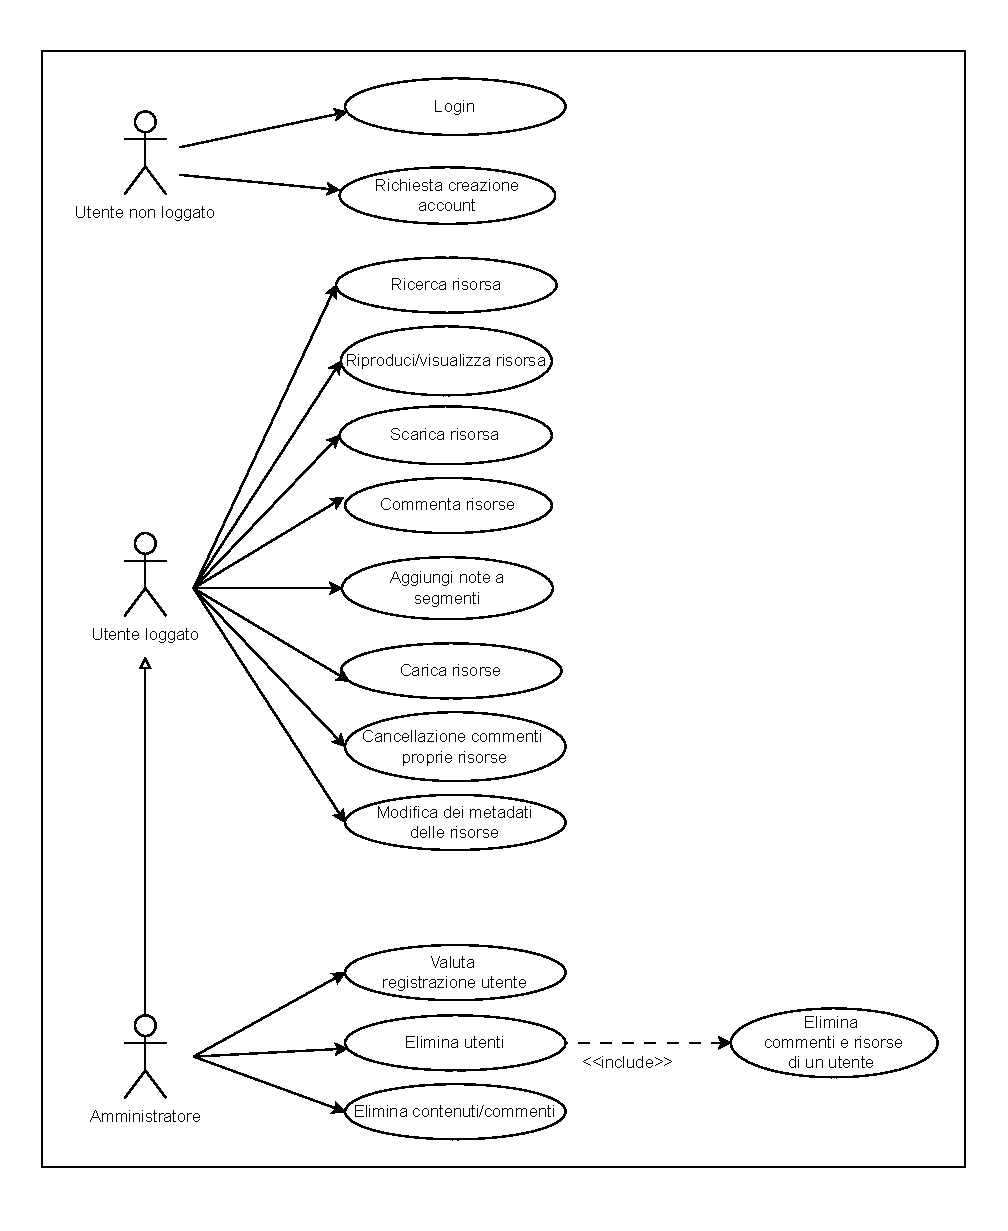
\includegraphics[width=0.8\textwidth]{./figures/use_cases}
    \caption{Use Cases}
    \label{fig:use_cases}
\end{figure}
\newpage
\subsubsection{Utente non loggato}
L'utente non autenticato può effettuare esclusivamente non operazioni:
    \begin{enumerate}
        \item Richiedere un account ad un amministratore
        \item Effettuare l'accesso tramite un form di autenticazione
    \end{enumerate}

\begin{table}[H]
\centering
\renewcommand{\arraystretch}{1.5}
\begin{tabular}{|>{\bfseries}l|p{10cm}|}
\hline
\multicolumn{2}{|c|}{\textbf{Caso d'uso: Login}} \\
\hline
\textbf{Id} & UC$0$ \\ \hline
\textbf{Attori} & Utente non loggato \\ \hline
\textbf{Precondizioni} & L’utente non è autenticato sulla piattaforma. \\ \hline
\textbf{Sequenza degli eventi} &
\begin{enumerate}
    \item L’utente compila i campi per effettuare l'autenticazione
    \item Il sistema verifica i dati e gestisce le autorizzazioni dell'utente
\end{enumerate}\\ \hline
\textbf{Post condizioni} & Utente autenticato e correttamente gestito \\ \hline
\end{tabular}
\caption{Descrizione caso d'uso \textit{Login}}
\label{tab:login-usecase}
\end{table}


\begin{table}[H]
    \centering
    \renewcommand{\arraystretch}{1.5}
    \begin{tabular}{|>{\bfseries}l|p{10cm}|}
        \hline
        \multicolumn{2}{|c|}{\textbf{Caso d'uso: Richiesta creazione account}} \\
        \hline
        \textbf{Id} & UC$1$ \\ \hline
        \textbf{Attori} & Utente non loggato \\ \hline
        \textbf{Precondizioni} & L’utente non è autenticato sulla piattaforma. \\
        & L’utente accede alla sezione di registrazione. \\ \hline % Added a new line and an empty cell for proper alignment
        \textbf{Sequenza degli eventi} &
        \begin{enumerate}
            \item Vengono compilati i dati relativi alla richiesta
            \item La richiesta viene inviata
            \item Il sistema registra la richiesta e la mette in stato di approvazione
            \item L'account viene salvato come account provvisorio
            \item Il sistema notifica l’amministratore della nuova richiesta
        \end{enumerate}\\ \hline
        \textbf{Sequenza alternativa } & Utente già esistente che comporta un messaggio di errore \\ \hline
        \textbf{Post condizioni} & La richiesta di creazione dell'account deve essere approvata da un amministratore \\ \hline
    \end{tabular}
    \caption{Descrizione caso d'uso \textit{Richiesta creazione account}}
    \label{tab:request_account-usecase}
\end{table}

\begin{figure}[H]
    \centering
    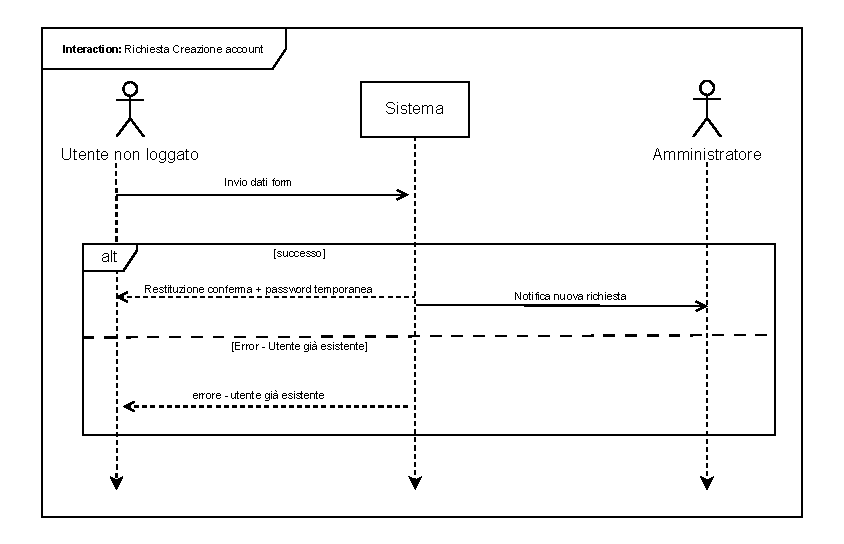
\includegraphics[width=0.9\textwidth]{./figures/account_request_sd}
    \caption{Sequence diagram del caso d'uso \textit{Richiesta creazione account}}
    \label{fig:sd_request_account}
\end{figure}

\subsubsection{Utente loggato}
\begin{table}[H]
    \centering
    \renewcommand{\arraystretch}{1.5}
    \begin{tabular}{|>{\bfseries}l|p{10cm}|}
        \hline
        \multicolumn{2}{|c|}{\textbf{Caso d'uso: Ricerca risorsa}} \\
        \hline
        \textbf{Id} & UC2 \\ \hline
        \textbf{Attori} & Utente loggato \\ \hline
        \textbf{Precondizioni} & Utente autenticato \\ \hline
        \textbf{Sequenza degli eventi} &
        \begin{enumerate}
            \item Il sistema invia i criteri di filtro disponibili
            \item L'utente decide il filtro di ricerca
            \item L'utente inserisce una parola chiave per ricercare una risorsa
            \item Gli vengono restituite le risorse data quella ricerca
        \end{enumerate}\\ \hline
        \textbf{Sequenza alternativa 1} & Errore nella ricerca: messaggio di errore \\ \hline
        \textbf{Post condizioni} & L'utente ha visualizzato la risorsa correttamente \\ \hline
    \end{tabular}
    \caption{Descrizione caso d'uso \textit{Ricerca risorsa}}
    \label{tab:search_resource-usecase}
\end{table}

\begin{figure}[H]
    \centering
    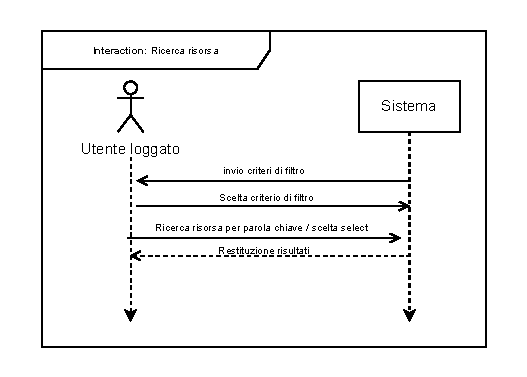
\includegraphics{./figures/ricerca_risorsa_sd}
    \caption{Sequence diagram del caso d'uso \textit{Ricerca risorsa}}
    \label{fig:sd_ricerca_risorsa}
\end{figure}

\begin{table}[H]
    \centering
    \renewcommand{\arraystretch}{1.5}
    \begin{tabular}{|>{\bfseries}l|p{10cm}|}
        \hline
        \multicolumn{2}{|c|}{\textbf{Caso d'uso: Riproduci/Visualizza risorsa}} \\
        \hline
        \textbf{Id} & UC3 \\ \hline
        \textbf{Attori} & User Logged \\ \hline
        \textbf{Precondizioni} &
        Utente autenticato \\& L'utente ha effettuato una ricerca o ne può selezionare una
        \\ \hline
        \textbf{Sequenza degli eventi} &
        \begin{enumerate}
            \item L'utente seleziona una risorsa dal risultato delle ricerca
            \item Il sistema riconosce il tipo di risorsa
            \item Se multimediale, lo riproduce
            \item Se testuale, lo visualizza
        \end{enumerate}\\ \hline
        \textbf{Sequenza alternativa 1} & Errore nella riproduzione: messaggio di errore \\ \hline
        \textbf{Post condizioni} & L'utente ha visualizzato la risorsa \\ \hline
    \end{tabular}
    \caption{Descrizione caso d'uso \textit{Riproduci/Visualizza risorsa}}
    \label{tab:play_view_resource-usecase}
\end{table}

\begin{figure}[H]
    \centering
    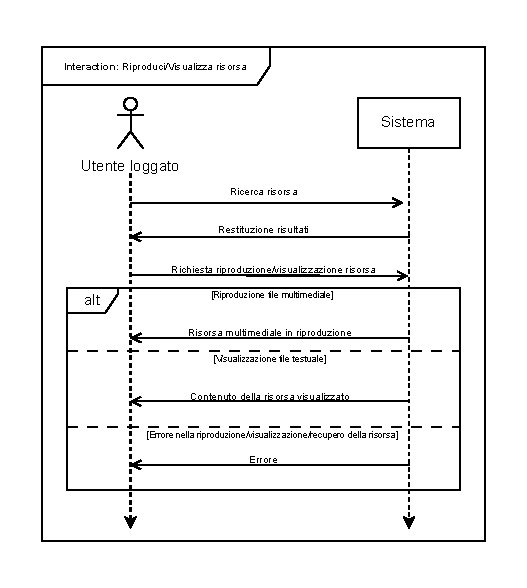
\includegraphics{./figures/visualizza_risorsa_sd}
    \caption{Sequence diagram del caso d'uso \textit{Riproduci/Visualizza risorsa}}
    \label{fig:sd_visualizza_risorsa}
\end{figure}

\begin{table}[H]
    \centering
    \renewcommand{\arraystretch}{1.5}
    \begin{tabular}{|>{\bfseries}l|p{10cm}|}
        \hline
        \multicolumn{2}{|c|}{\textbf{Caso d'uso: Scarica risorsa}} \\
        \hline
        \textbf{Id} & UC4 \\ \hline
        \textbf{Attori} & User Logged \\ \hline
        \textbf{Precondizioni} & Utente autenticato \\
        & L'utente ha effettuato una ricerca o ne può selezionare una \\ \hline
        \textbf{Sequenza degli eventi} &
        \begin{enumerate}
            \item L'utente seleziona una risorsa dal risultato delle ricerca
            \item L'utente richiede il download della risorsa
        \end{enumerate}\\ \hline
        \textbf{Sequenza alternativa 1} & Errore nel download: messaggio di errore \\ \hline
        \textbf{Post condizioni} & L'utente ha scaricato la risorsa correttamente \\ \hline
    \end{tabular}
    \caption{Descrizione caso d'uso \textit{Scarica risorsa}}
    \label{tab:download_resource-usecase}
\end{table}

\begin{figure}[H]
    \centering
    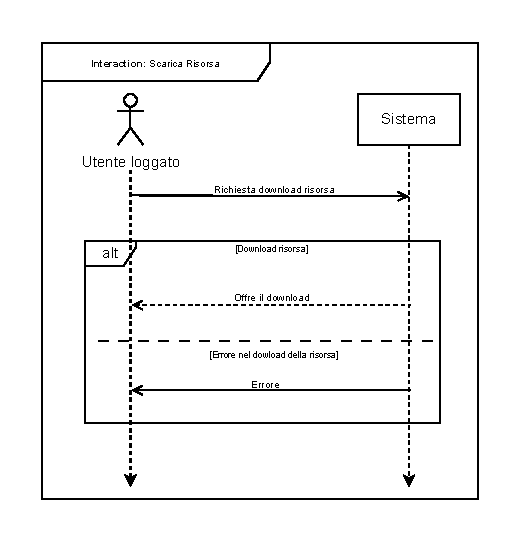
\includegraphics{./figures/scarica_sd}
    \caption{Sequence diagram del caso d'uso \textit{Scarica risorsa}}
    \label{fig:sd_download_resource}
\end{figure}

\begin{table}[H]
    \centering
    \renewcommand{\arraystretch}{1.5}
    \begin{tabular}{|>{\bfseries}l|p{10cm}|}
        \hline
        \multicolumn{2}{|c|}{\textbf{Caso d'uso: Commenta risorse}} \\
        \hline
        \textbf{Id} & UC5 \\ \hline
        \textbf{Attori} & User Logged \\ \hline
        \textbf{Precondizioni} & Utente autenticato \\
        & L'utente può visualizzare una risorsa \\ \hline
        \textbf{Sequenza degli eventi} &
        \begin{enumerate}
            \item L'utente seleziona una risorsa dal risultato delle ricerca
            \item L'utente può scrivere un commento
            \item Il commento viene salvato dal sistema
        \end{enumerate}\\ \hline
        \textbf{Sequenza alternativa 1} & L'utente può rispondere ad un commento \\ \hline
        \textbf{Post condizioni} & L'utente ha commentato la risorsa correttamente \\ \hline
    \end{tabular}
    \caption{Descrizione caso d'uso \textit{Commenta risorse}}
    \label{tab:comment_resource-usecase}
\end{table}

\begin{figure}[H]
    \centering
    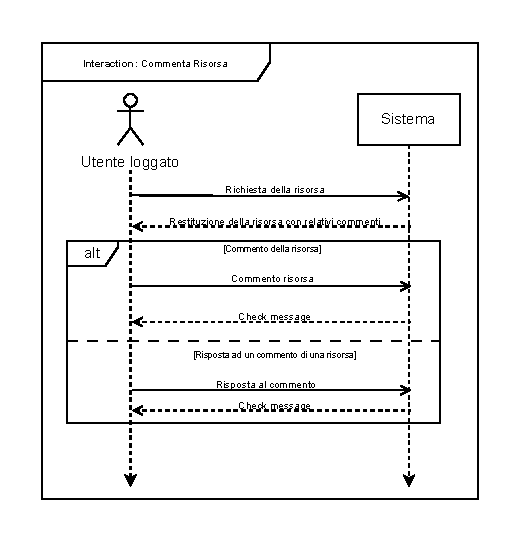
\includegraphics{./figures/commenta_risorsa_sd}
    \caption{Sequence diagram del caso d'uso \textit{Commenta risorse}}
    \label{fig:sd_commenta_risorsa}
\end{figure}

\begin{table}[H]
    \centering
    \renewcommand{\arraystretch}{1.5}
    \begin{tabular}{|>{\bfseries}l|p{10cm}|}
        \hline
        \multicolumn{2}{|c|}{\textbf{Caso d'uso: Aggiungi note a segmenti}} \\
        \hline
        \textbf{Id} & UC6 \\ \hline
        \textbf{Attori} & User Logged \\ \hline
        \textbf{Precondizioni} & Utente autenticato \\
        & L'utente ha ricercato/può visualizzare una risorsa \\ \hline
        \textbf{Sequenza degli eventi} &
        \begin{enumerate}
            \item L'utente seleziona un intervallo di tempo per inserire una nota/commento
            \item Scrive la /commento desiderata
            \item Invia la nota/commento al sistema
            \item Il sistema registra la nota/commento
        \end{enumerate}\\ \hline
        \textbf{Post condizioni} & L'utente ha scritto una nota/commento su un segmento correttamente \\ \hline
    \end{tabular}
    \caption{Descrizione caso d'uso \textit{Aggiungi note a segmenti}}
    \label{tab:add_notes_to_segments-usecase}
\end{table}


\begin{table}[H]
    \centering
    \renewcommand{\arraystretch}{1.5}
    \begin{tabular}{|>{\bfseries}l|p{10cm}|}
        \hline
        \multicolumn{2}{|c|}{\textbf{Caso d'uso: Carica Risorse}} \\
        \hline
        \textbf{Id} & UC7 \\ \hline
        \textbf{Attori} & User Logged \\ \hline
        \textbf{Precondizioni} & Utente autenticato \\ \hline
        \textbf{Sequenza degli eventi} &
        \begin{enumerate}
            \item L'utente visualizza la schermata di upload dei file
            \item Seleziona la risorsa da caricare
            \item Inserisce i dati (file + metadati obbligatori)
            \item Invia i dati al sistema
            \item Il sistema li memorizza
        \end{enumerate}\\ \hline
        \textbf{Sequenza alternativa 1} & Errore di sistema: messaggio di errore \\ \hline
        \textbf{Sequenza alternativa 2} & Errore nell'inserimento dei dati: messaggio di errore \\ \hline
        \textbf{Post condizioni} & L'utente ha caricato la risorsa correttamente \\ \hline
    \end{tabular}
    \caption{Descrizione caso d'uso \textit{Carica Risorse}}
    \label{tab:upload_resources-usecase}
\end{table}

\begin{figure}[H]
    \centering
    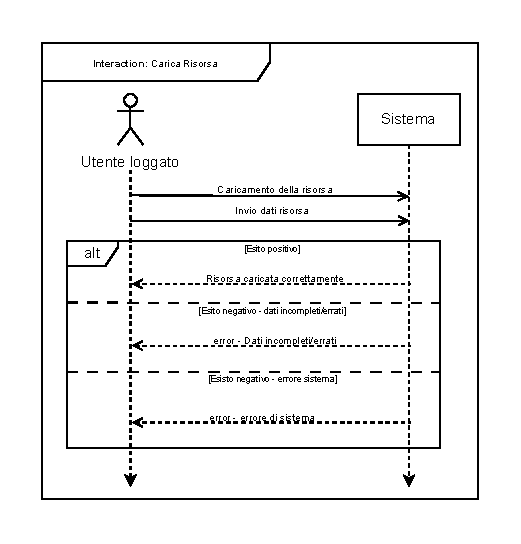
\includegraphics{./figures/carica_risorsa_sd}
    \caption{Sequence diagram del caso d'uso \textit{Carica Risorse}}
    \label{fig:sd_carica_risorsa}
\end{figure}

\begin{table}[H]
    \centering
    \renewcommand{\arraystretch}{1.5}
    \begin{tabular}{|>{\bfseries}l|p{10cm}|}
        \hline
        \multicolumn{2}{|c|}{\textbf{Caso d'uso: Cancellazione commenti delle proprie risorse}} \\
        \hline
        \textbf{Id} & UC8 \\ \hline
        \textbf{Attori} & User Logged \\ \hline
        \textbf{Precondizioni} & Utente autenticato e autorizzato \\
        & L'utente sta visualizzando una propria risorsa caricata \\ \hline
        \textbf{Sequenza degli eventi} &
        \begin{enumerate}
            \item L'utente desidera eliminare un qualsiasi commento della risorsa
            \item Elimina il commento
            \item Il sistema controlla che abbia i permessi necessari
            \item In caso positivo effettua la rimozione
            \item Vengono rimossi tutte le risposte a quel commento
        \end{enumerate}\\ \hline
        \textbf{Sequenza alternativa 1} & Errore Autorizzazioni: messaggio di errore \\ \hline
        \textbf{Post condizioni} & L'utente ha eliminato il commento correttamente \\ \hline
    \end{tabular}
    \caption{Descrizione caso d'uso \textit{Cancellazione commenti delle proprie risorse}}
    \label{tab:delete_comments_own_resources-usecase}
\end{table}

\begin{table}[H]
    \centering
    \renewcommand{\arraystretch}{1.5}
    \begin{tabular}{|>{\bfseries}l|p{10cm}|}
        \hline
        \multicolumn{2}{|c|}{\textbf{Caso d'uso: Modifica dei metadati delle risorse}} \\
        \hline
        \textbf{Id} & UC9 \\ \hline
        \textbf{Attori} & User Logged Authorized \\ \hline
        \textbf{Precondizioni} & Utente autenticato \\
        & L'utente è il proprietario di quella risorsa \\
        & L'utente sta visualizzando i dati di una risorsa \\ \hline
        \textbf{Sequenza degli eventi} &
        \begin{enumerate}
            \item L'utente desidera modificare un qualsiasi metadato della risorsa
            \item Modifica i metadati
            \item Invia le modifiche al sistema
            \item Il sistema effettua la modifica
        \end{enumerate}\\ \hline
        \textbf{Post condizioni} & L'utente ha modificato correttamente i metadati di una risorsa \\ \hline
    \end{tabular}
    \caption{Descrizione caso d'uso \textit{Modifica dei metadati delle risorse}}
    \label{tab:modify_metadata_uc9-usecase}
\end{table}

    \subsubsection{Amministratore}
\begin{table}[H]
    \centering
    \renewcommand{\arraystretch}{1.5}
    \begin{tabular}{|>{\bfseries}l|p{10cm}|}
        \hline
        \multicolumn{2}{|c|}{\textbf{Caso d'uso: Valuta registrazione utente}} \\
        \hline
        \textbf{Id} & UC10 \\ \hline
        \textbf{Attori} & Administrator \\ \hline
        \textbf{Precondizioni} & L'amministratore accede alla sezione di gestione delle registrazioni utente in attesa di valutazione \\ \hline
        \textbf{Sequenza degli eventi} &
        \begin{enumerate}
            \item L'amministratore visualizza i dettagli
            \item L'amministratore approva/rifiuta la richiesta
            \item Il sistema elimina la richiesta e in caso di approvazione crea l'account
            \item Il sistema notifica all'utente l'esito
        \end{enumerate}\\ \hline
        \textbf{Post condizioni} & L'utente è registrato e abilitato all'accesso al sistema (se approvato) o la sua richiesta di registrazione viene rifiutata \\ \hline
    \end{tabular}
    \caption{Descrizione caso d'uso \textit{Valuta registrazione utente}}
    \label{tab:evaluate_user_registration-usecase}
\end{table}

\begin{figure}[H]
    \centering
    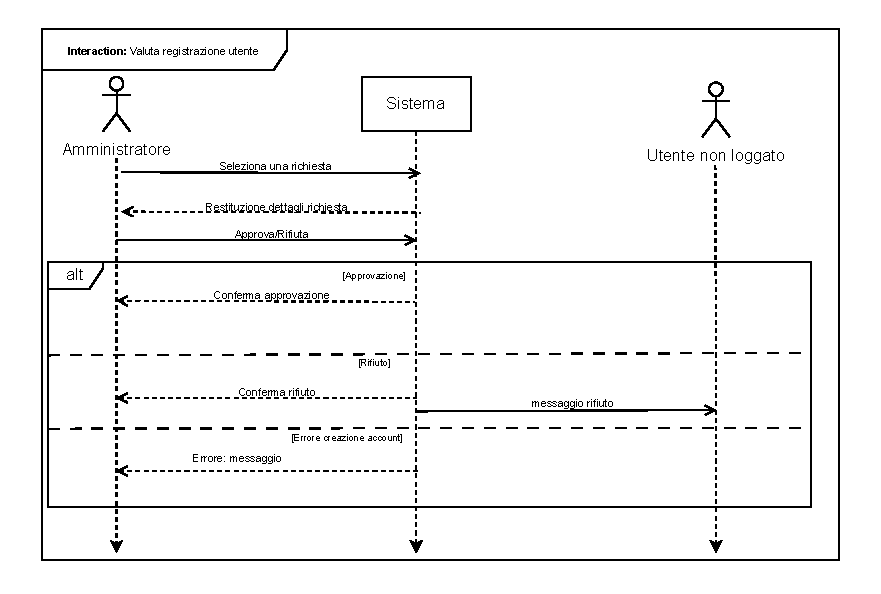
\includegraphics{./figures/valuta_richieste}
    \caption{Sequence diagram del caso d'uso \textit{Valuta registrazione utente}}
    \label{fig:sd_valuta_richiesta}
\end{figure}

\begin{table}[H]
    \centering
    \renewcommand{\arraystretch}{1.5}
    \begin{tabular}{|>{\bfseries}l|p{10cm}|}
        \hline
        \multicolumn{2}{|c|}{\textbf{Caso d'uso: Eliminazione utente}} \\
        \hline
        \textbf{Id} & UC11 \\ \hline
        \textbf{Attori} & Administrator \\ \hline
        \textbf{Precondizioni} & L'amministratore accede alla sezione di gestione degli utenti \\ \hline
        \textbf{Sequenza degli eventi} &
        \begin{enumerate}
            \item L'amministratore seleziona l'utente che desidera eliminare
            \item L'amministratore elimina l'utente
            \item Rimuove l'utente
        \end{enumerate}\\ \hline
        \textbf{Post condizioni} & L'utente è stato cancellato correttamente \\ \hline
    \end{tabular}
    \caption{Descrizione caso d'uso \textit{Eliminazione utente}}
    \label{tab:delete_user-usecase}
\end{table}

\begin{table}[H]
    \centering
    \renewcommand{\arraystretch}{1.5}
    \begin{tabular}{|>{\bfseries}l|p{10cm}|}
        \hline
        \multicolumn{2}{|c|}{\textbf{Caso d'uso: Elimina commenti e risorse di un utente}} \\
        \hline
        \textbf{Id} & UC12 \\ \hline
        \textbf{Attori} & Administrator \\ \hline
        \textbf{Precondizioni} & Caso d'uso \textit{Eliminazine Utente} (\autoref{tab:delete_user-usecase}) \\ \hline
        \textbf{Sequenza degli eventi} &
        \begin{enumerate}
            \item L'amministratore comunica al server un utente
            \item Le risorse e commenti di questo utente vengono eliminate
        \end{enumerate}\\ \hline
        \textbf{Post condizioni} & Le risorse/commenti sono stati cancellati correttamente \\ \hline
    \end{tabular}
    \caption{Descrizione caso d'uso \textit{Elimina commenti e risorse di un utente}}
    \label{tab:delete_user_comments_resources-usecase}
\end{table}

\begin{table}[H]
    \centering
    \renewcommand{\arraystretch}{1.5}
    \begin{tabular}{|>{\bfseries}l|p{10cm}|}
        \hline
        \multicolumn{2}{|c|}{\textbf{Caso d'uso: Elimina contenuti/commenti}} \\
        \hline
        \textbf{Id} & UC13 \\ \hline
        \textbf{Attori} & Administrator \\ \hline
        \textbf{Precondizioni} & Visualizzazione di una risorsa/commento \\ \hline
        \textbf{Sequenza degli eventi} &
        \begin{enumerate}
            \item L'amministratore visualizza una risorsa
            \item L'amministratore decide di eliminare la risorsa/commento
            \item Invia la richiesta al sistema
            \item Il sistema elimina la risorsa/commento
        \end{enumerate}\\ \hline
        \textbf{Post condizioni} & La risorsa/commento è stata eliminata correttamente \\ \hline
    \end{tabular}
    \caption{Descrizione caso d'uso \textit{Elimina contenuti/commenti}}
    \label{tab:delete_content_comments-usecase}
\end{table}


\subsection{Glossario dei termini}

\begin{table}[H]
    \centering
    \renewcommand{\arraystretch}{1.5}
    % Modifica qui:
    % Ad esempio, la prima colonna l'ho fatta p{0.25\textwidth}
    % e la seconda p{0.65\textwidth}. La somma (0.25+0.65=0.90) lascia spazio per i bordi e tabcolsep.
    \begin{tabular}{|>{\bfseries}p{0.28\textwidth}|p{0.62\textwidth}|}
        \hline
        \multicolumn{2}{|c|}{\textbf{GLOSSARIO DEI TERMINI}} \\
        \hline
        \textbf{TERMINE} & \textbf{DEFINIZIONE} \\
        \hline
        Contenuto musicale / Risorsa multimediale & Qualsiasi tipo di file audio, video o immagine caricato e reso disponibile sulla piattaforma. Può includere brani musicali, podcast, lezioni, video, ecc. \\
        \hline
        Autore / Esecutore / Interprete di un brano & L'individuo o il gruppo che ha contribuito in modo significativo alla creazione, composizione, esecuzione o interpretazione originale di un'opera musicale. \\
        \hline
        Segmento di un brano & Un sottoinsieme specifico di un contenuto multimediale (es. un brano musicale o un video), definito da un intervallo di tempo di inizio e fine, permettendo di focalizzare l'attenzione su una parte specifica. \\
        \hline
        Traccia & Una traccia può contenere più risorse relative a quel contesto, ad esempio il relativo file PDF dello spartito + un'eventuale risorsa multimediale (mp4/mp3) \\
        \hline
        Brano & Un'opera musicale originale completa e autonoma, che può essere parte di un album o una singola traccia, caratterizzata da una composizione unica. \\
        \hline
        Metadato & Un insieme di dati che descrivono e forniscono informazioni su altri dati (una risorsa). Per un brano, i metadati possono includere titolo, autore, genere, durata, data di pubblicazione, ecc. \\
        \hline
        Utente autenticato / Loggato & Un utente che ha completato con successo il processo di login fornendo credenziali valide ed è riconosciuto dal sistema, avendo accesso a funzionalità riservate. \\
        \hline
        Amministratore & Un utente con privilegi speciali all'interno della piattaforma, in grado di gestire utenti, contenuti, approvare richieste e monitorare le operazioni del sistema. \\
        \hline
        Richiesta di creazione account & La procedura iniziata da un utente non autenticato per ottenere un nuovo account sulla piattaforma, soggetta ad approvazione da parte di un amministratore. \\
        \hline
        Commento & Un testo o una nota aggiunta da un utente autenticato a una risorsa (o a un altro commento) per esprimere un'opinione, fornire feedback o interagire con altri utenti. \\
        \hline
        Nota a segmento & Un tipo specifico di commento o annotazione testuale associata a un intervallo di tempo preciso all'interno di una risorsa multimediale, permettendo di evidenziare o commentare una parte specifica del contenuto. \\
        \hline
    \end{tabular}
    \caption{Glossario dei Termini}
    \label{tab:glossary}
\end{table}

\subsection{Activity Diagrams}
Questa sezione illustra i principali flussi di lavoro del sistema attraverso gli activity diagrams.

\begin{figure}[H]
    \centering
    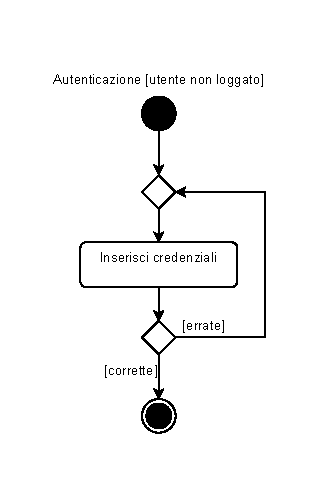
\includegraphics{./figures/autenticazione_ac}
    \caption{Activity Diagrams del caso d'uso \textit{Login}}
    \label{fig:ac_login}
\end{figure}

\begin{figure}[H]
    \centering
    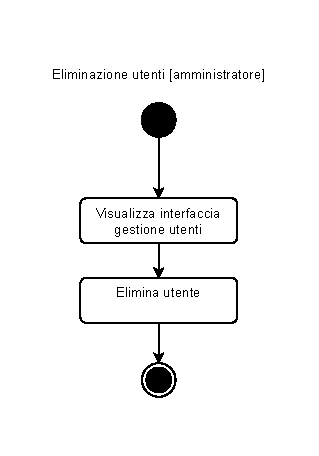
\includegraphics{./figures/eliminazione_utenti_ac}
    \caption{Activity Diagrams del caso d'uso \textit{Elimina utenti}}
    \label{fig:ac_eliminazione_utenti}
\end{figure}

\begin{figure}[H]
    \centering
    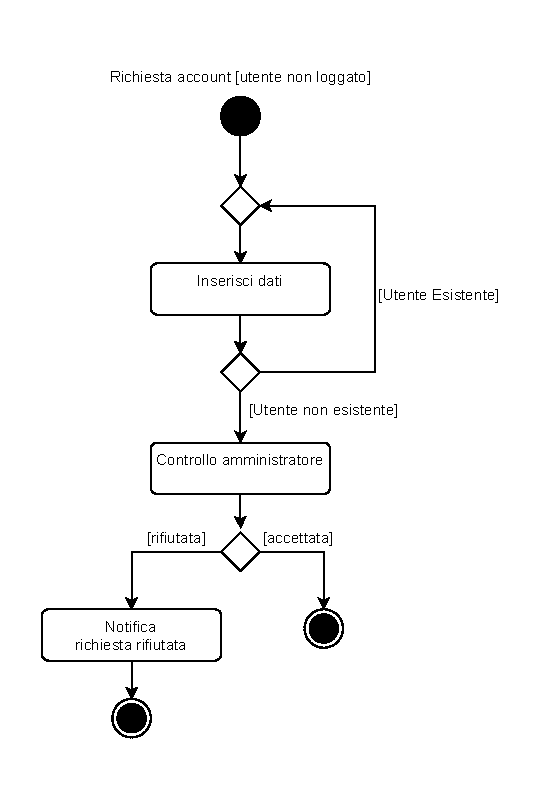
\includegraphics{./figures/account_request_ac}
    \caption{Activity Diagrams del caso d'uso \textit{Richiesta creazione account}}
    \label{fig:ac_account_request}
\end{figure}

\begin{figure}[H]
    \centering
    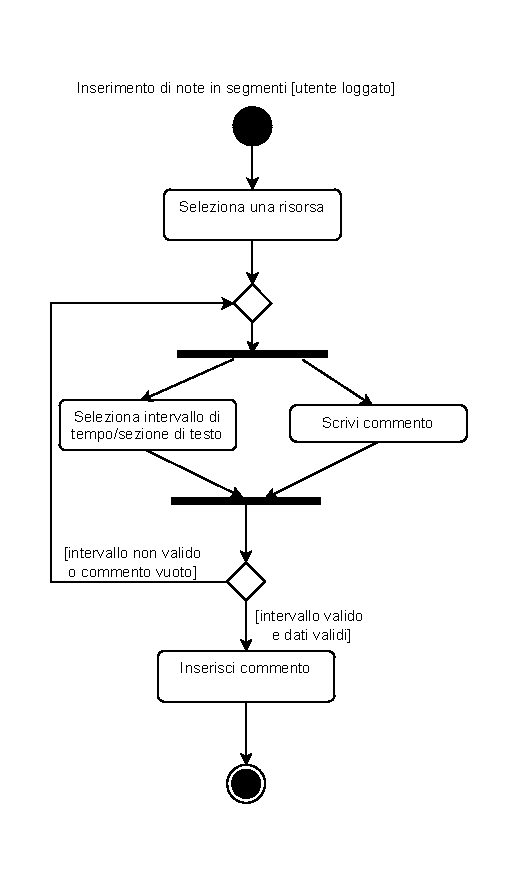
\includegraphics{./figures/segmenti_commenti_ac}
    \caption{Activity Diagrams del caso d'uso \textit{Aggiungi note a segmenti}}
    \label{fig:ac_note_segmenti}
\end{figure}

\begin{figure}[H]
    \centering
    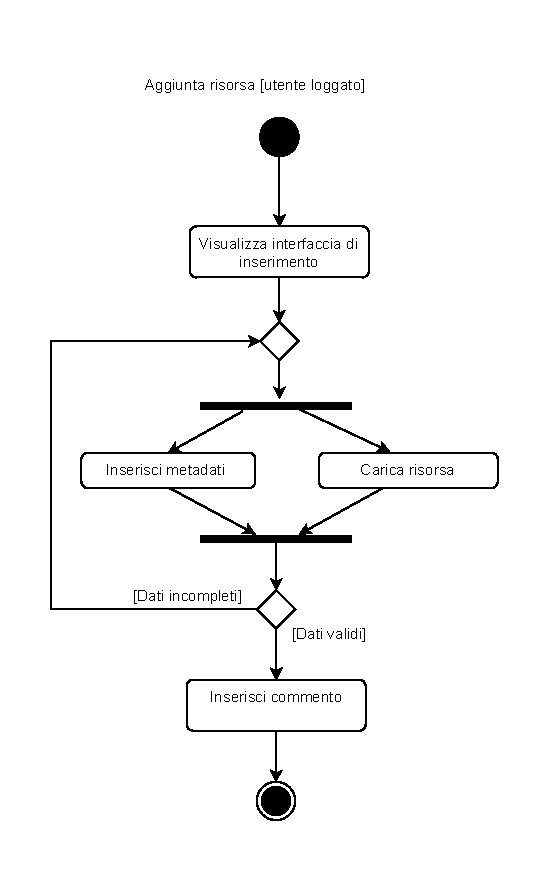
\includegraphics{./figures/aggiungi_risorsa_ac}
    \caption{Activity Diagrams del caso d'uso \textit{Carica risorse}}
    \label{fig:ac_valuta_registrazione_utenti}
\end{figure}

\begin{figure}[H]
    \centering
    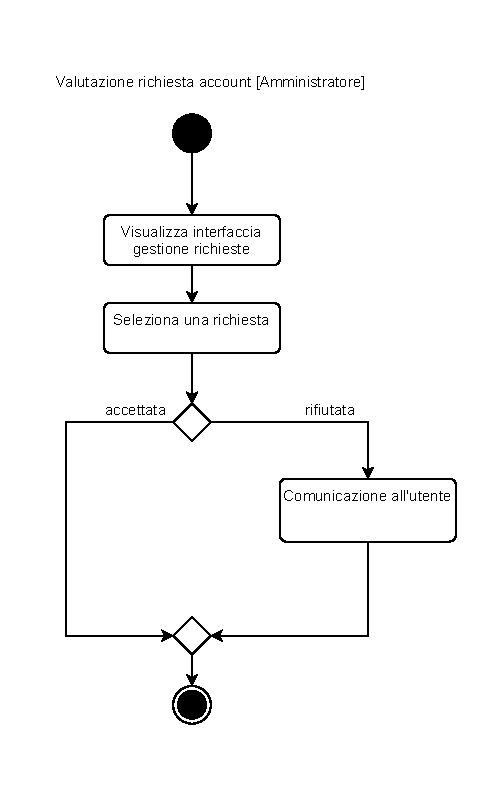
\includegraphics{./figures/valutazione_richiesta_ac}
    \caption{Activity Diagrams del caso d'uso \textit{Valuta registrazione utenti}}
    \label{fig:ac_carica_risorsa}
\end{figure}

% =======================
\section{Modello logico dei dati}
La presente sezione descrive il modello logico dei dati adottato nel sistema, che rappresenta l’organizzazione e la struttura concettuale
delle informazioni da gestire.

% =======================
\subsection{Diagramma E/R}
\begin{figure}[H]
    \centering
    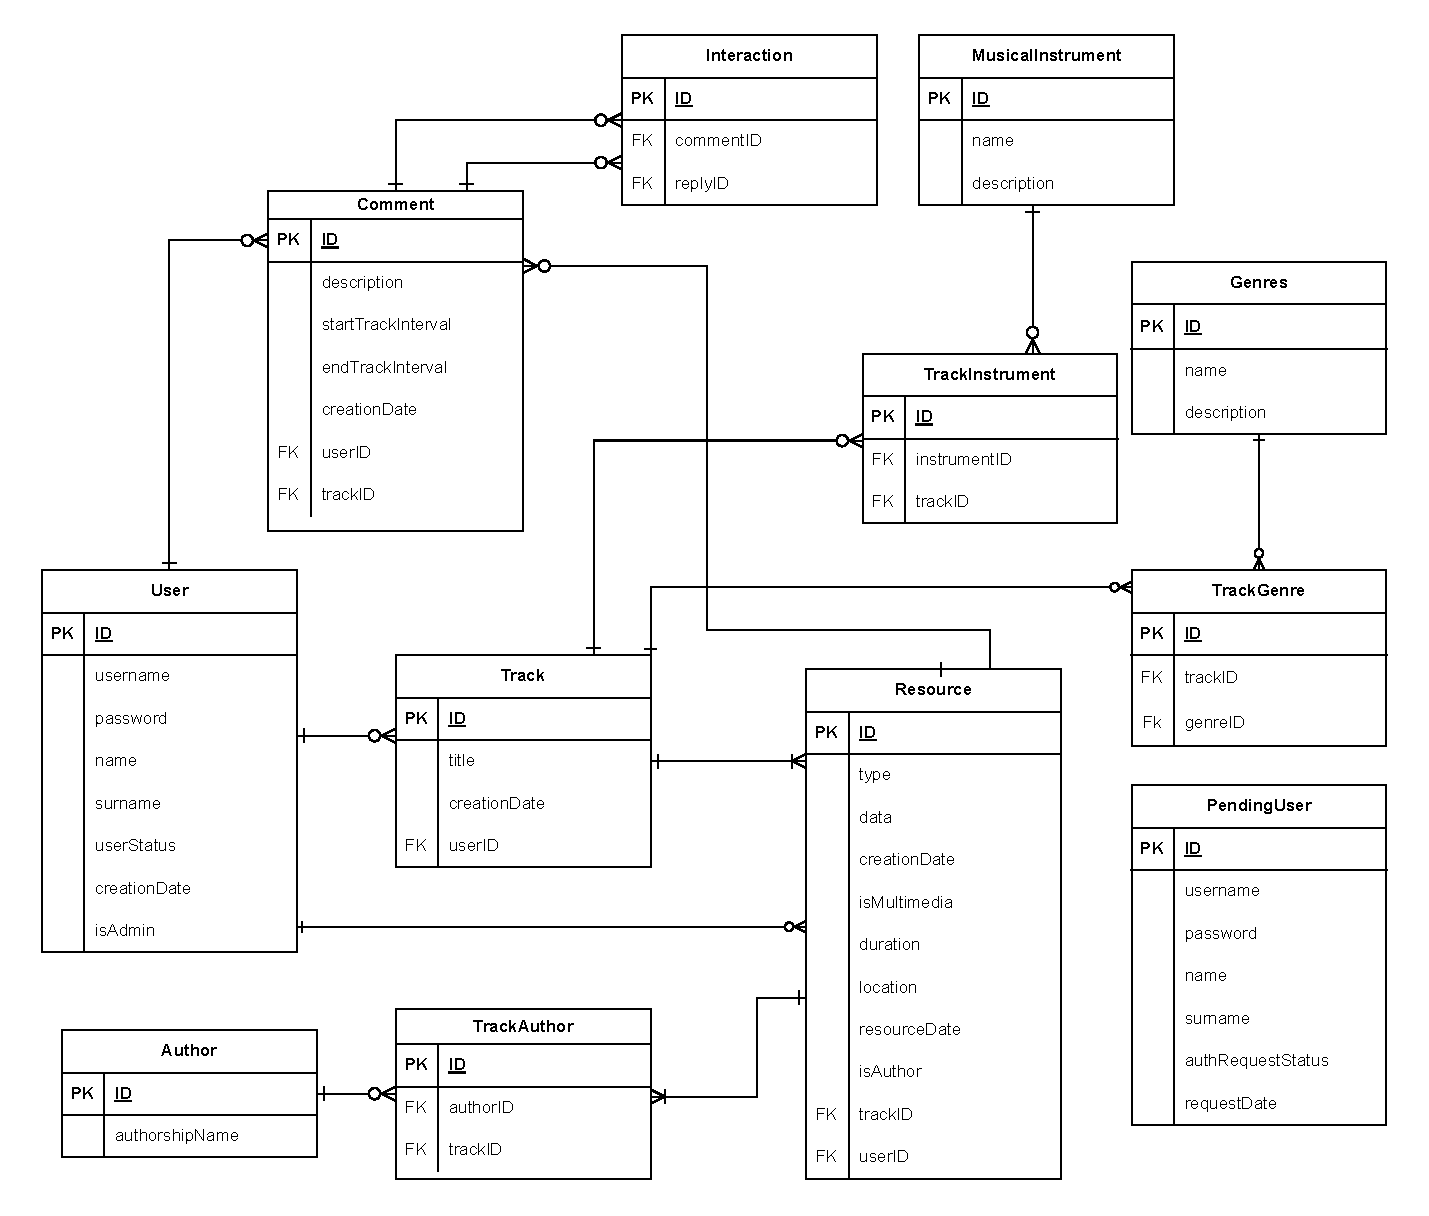
\includegraphics[width=1.1 \textwidth]{./figures/diagramma_er_ristrutturato}
    \caption{Diagramma E/R ristrutturato}
    \label{fig:er_ristrutturato}
\end{figure}

% =======================
\section{Architettura logica}
% =======================
Questa sezione presenta l’architettura logica del sistema, ovvero come sono organizzati i principali componenti software e come interagiscono tra loro. L’obiettivo è offrire una panoramica chiara della struttura del progetto, utile per guidare lo sviluppo e facilitare la manutenzione nel tempo.

\subsection{Diagramma UML delle classi - Model}
\begin{figure}[H]
    \centering
    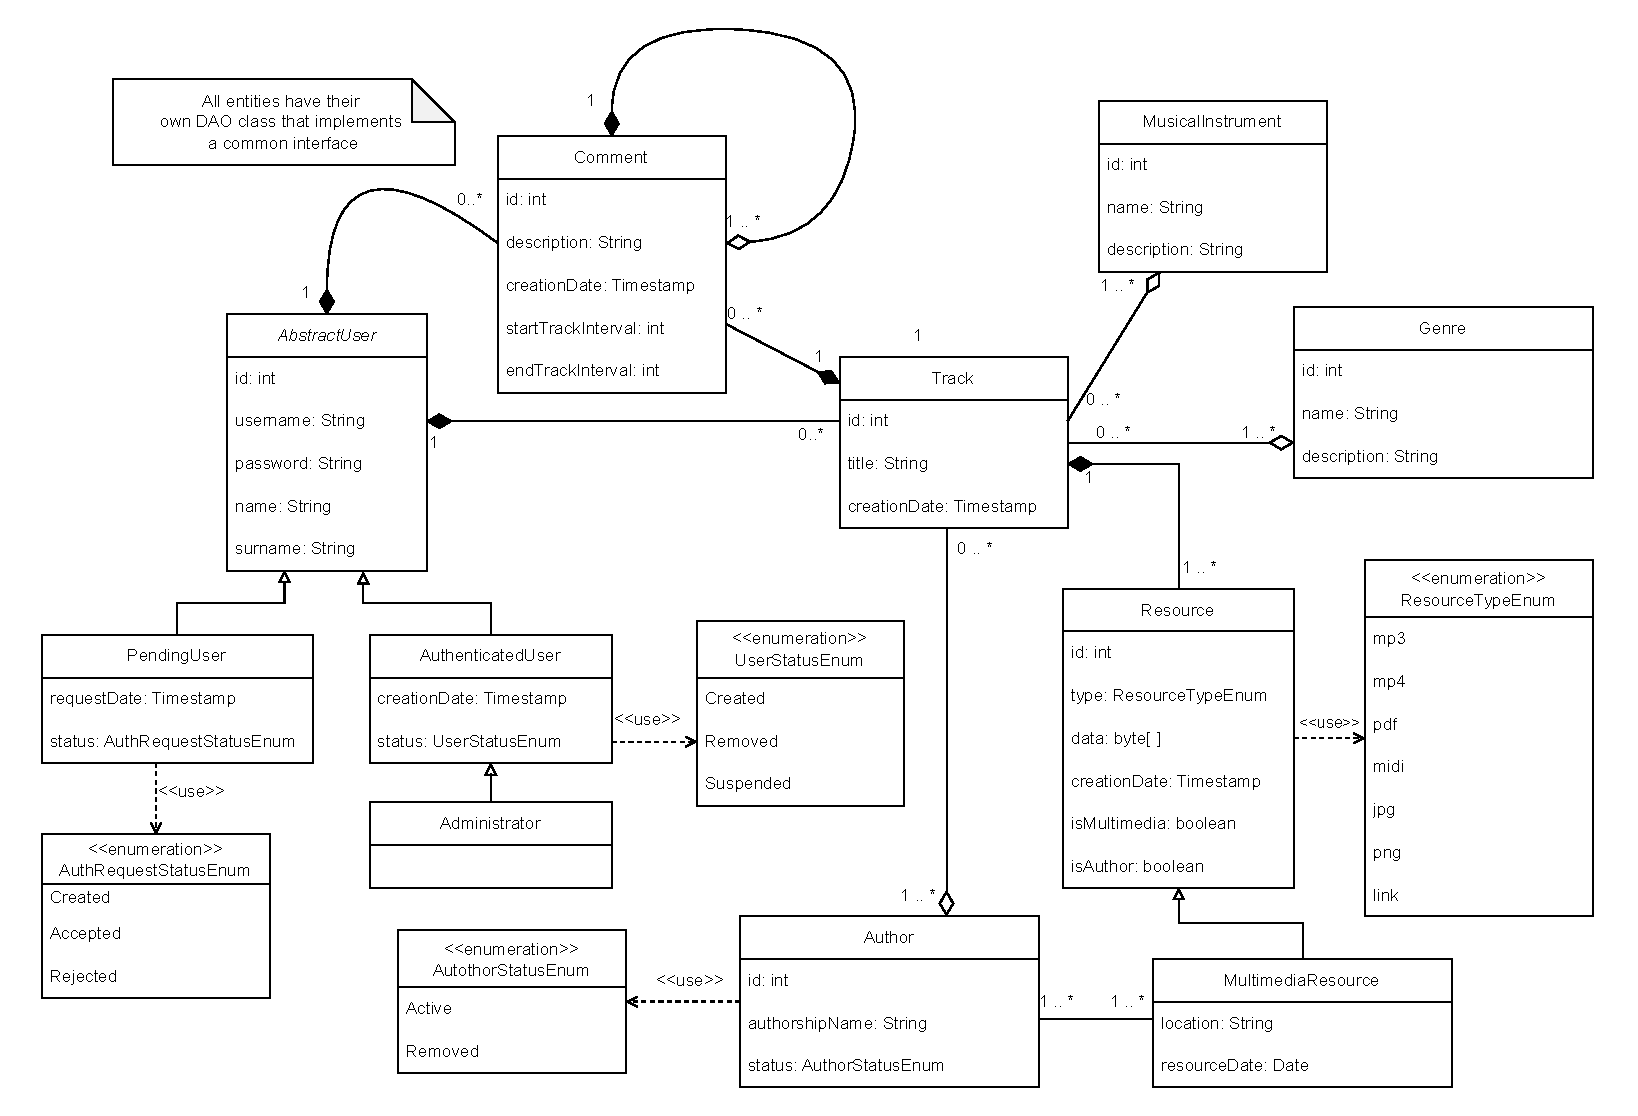
\includegraphics[width=1.1 \textwidth]{./figures/uml_table_model}
    \caption{Class Diagrams UML relative al \textit{Model}}
    \label{fig:uml_table_model}
\end{figure}

\subsection{Diagramma UML delle classi - Control}
\begin{figure}[H]
    \centering
    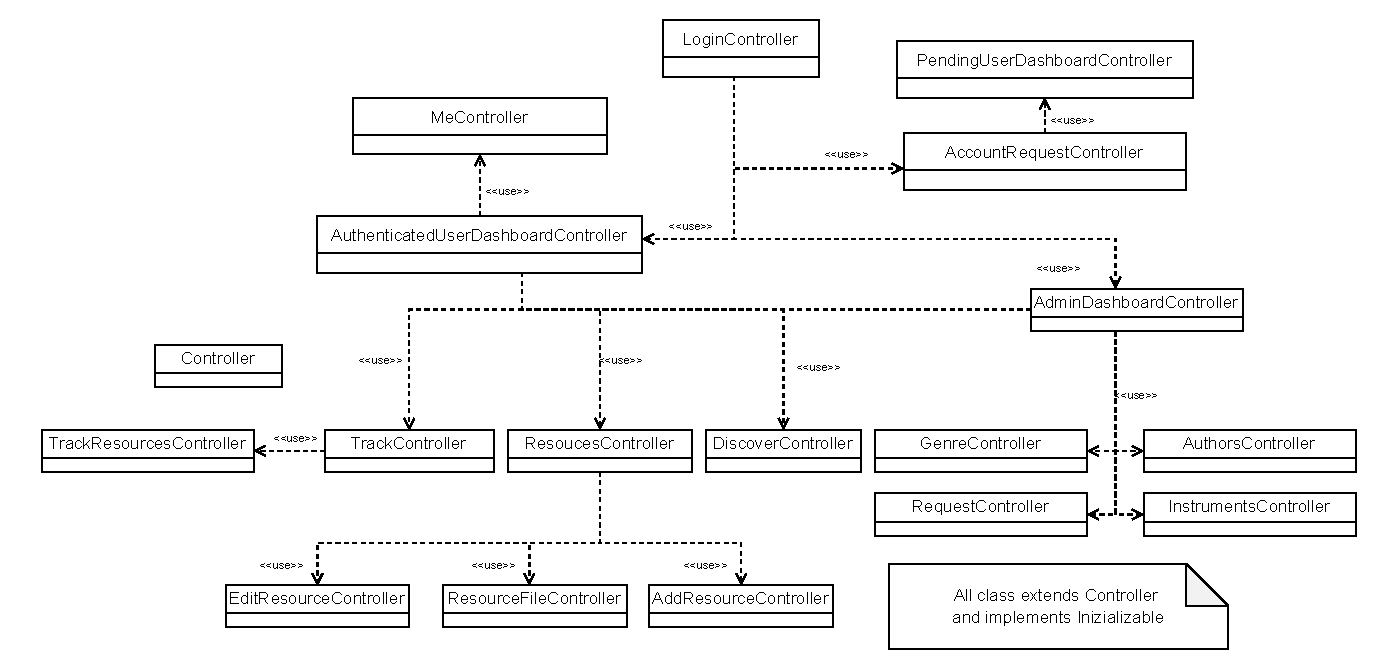
\includegraphics[width=1.1 \textwidth]{./figures/uml_table_controller}
    \caption{Class Diagrams UML relative al \textit{Controller}}
    \label{fig:uml_table_controller}
\end{figure}

Il diagramma mostra la classe base \texttt{Controller} e tutte le sue sottoclassi organizzate nei seguenti pacchetti:
\begin{lstlisting}[style=filetree]
Controller
  common
    AddResourceController
    DiscoverController
    EditResourceController
    ResourceFileController
    ResourcesController
    TrackResourcesController
    TracksController
  admin
    AdminDashboardController
    AuthorsController
    GenresController
    InstrumentsController
    RequestsController
    UsersController
  authenticatedUser
    AuthenticatedUserDashboardController
    MeController
  authentication
    AccountRequestController
    LoginController
    SessionManager
  pendingUser
    PendingUserDashboardController
\end{lstlisting}


Tutte le classi controller estendono la classe base \texttt{Controller} e implementano l'interfaccia \texttt{Initializable} di JavaFX.

\subsection{Diagramma UML delle classi - Utility ed Exception}
\begin{figure}[H]
    \centering
    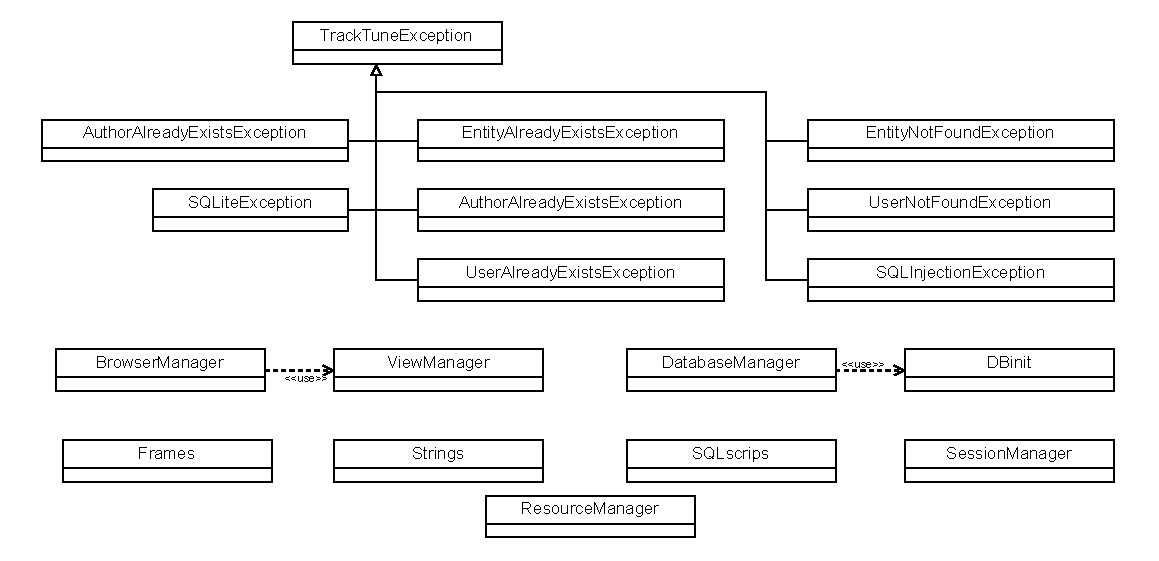
\includegraphics[width=1.1 \textwidth]{./figures/uml_table_altri_package}
    \caption{Class Diagrams UML relative a \textit{Utility ed Exception}}
    \label{fig:uml_table_altri_package}
\end{figure}

\subsection{Struttura del progetto}

Di seguito è riportato l’albero dei file principali del progetto, illustrante la suddivisione in moduli, package e risorse:

\begin{lstlisting}[style=filetree]
TrackTune/
  src/
    main/
      java/                   % codice sorgente principale
        app/tracktune/
          config/
          controller/
          exception/
          interfaces/
          model/
          utils/
            DatabaseManager.java
            DBInit.java
          view/
          Main.java
      resources/               % FXML, CSS, immagini
    test/                     % test automatici (JUnit)
pom.xml                      % file di build Maven
\end{lstlisting}

\subsection{Sequence Diagrams}
I diagrammi di sequenza sono rappresentati esclusivamente per le classi più rilevanti e significative del sistema.

\begin{figure}[H]
    \centering
    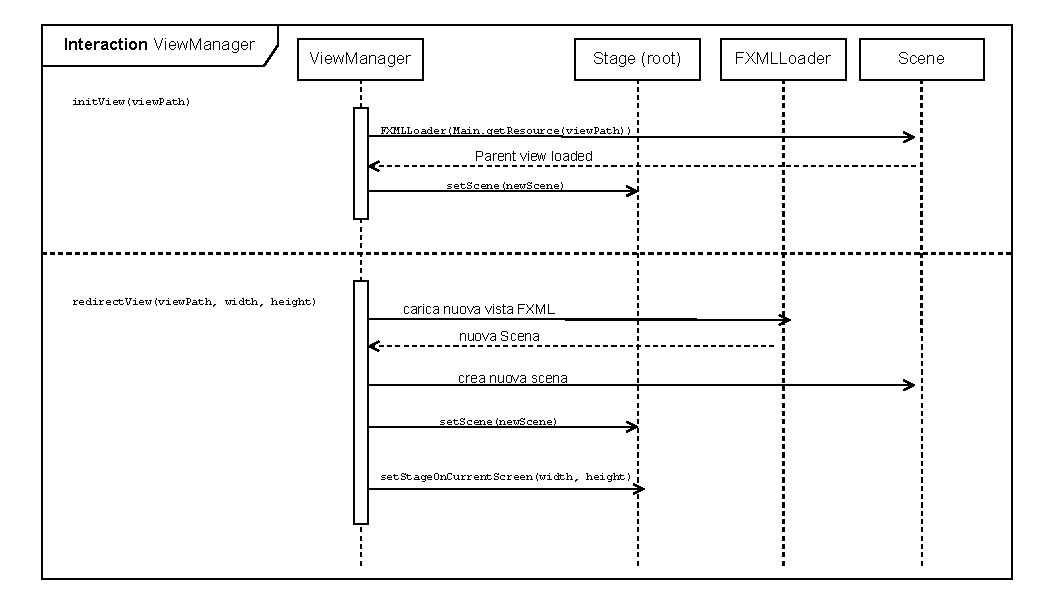
\includegraphics[width=0.8\textwidth]{./figures/viewManager_sd}
    \caption{Sequence diagram relavito alla classe \texttt{ViewManager.java} in particolare al cambio di scena e inizializzazione root iniziale}
    \label{fig:viewmanager_sd}
\end{figure}

\begin{figure}[H]
    \centering
    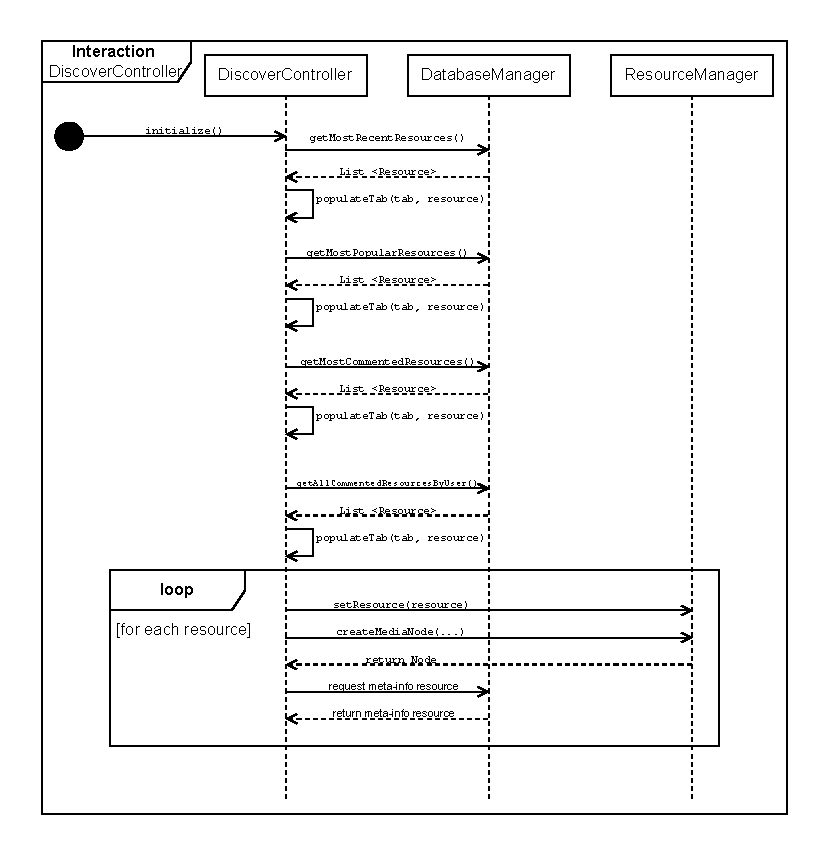
\includegraphics[width=0.8 \textwidth]{./figures/discoverController_sd}
    \caption{Sequence diagram relavito alla classe \texttt{DiscoverController.java}}
    \label{fig:discovercontroller_sd}
\end{figure}

\begin{figure}[H]
    \centering
    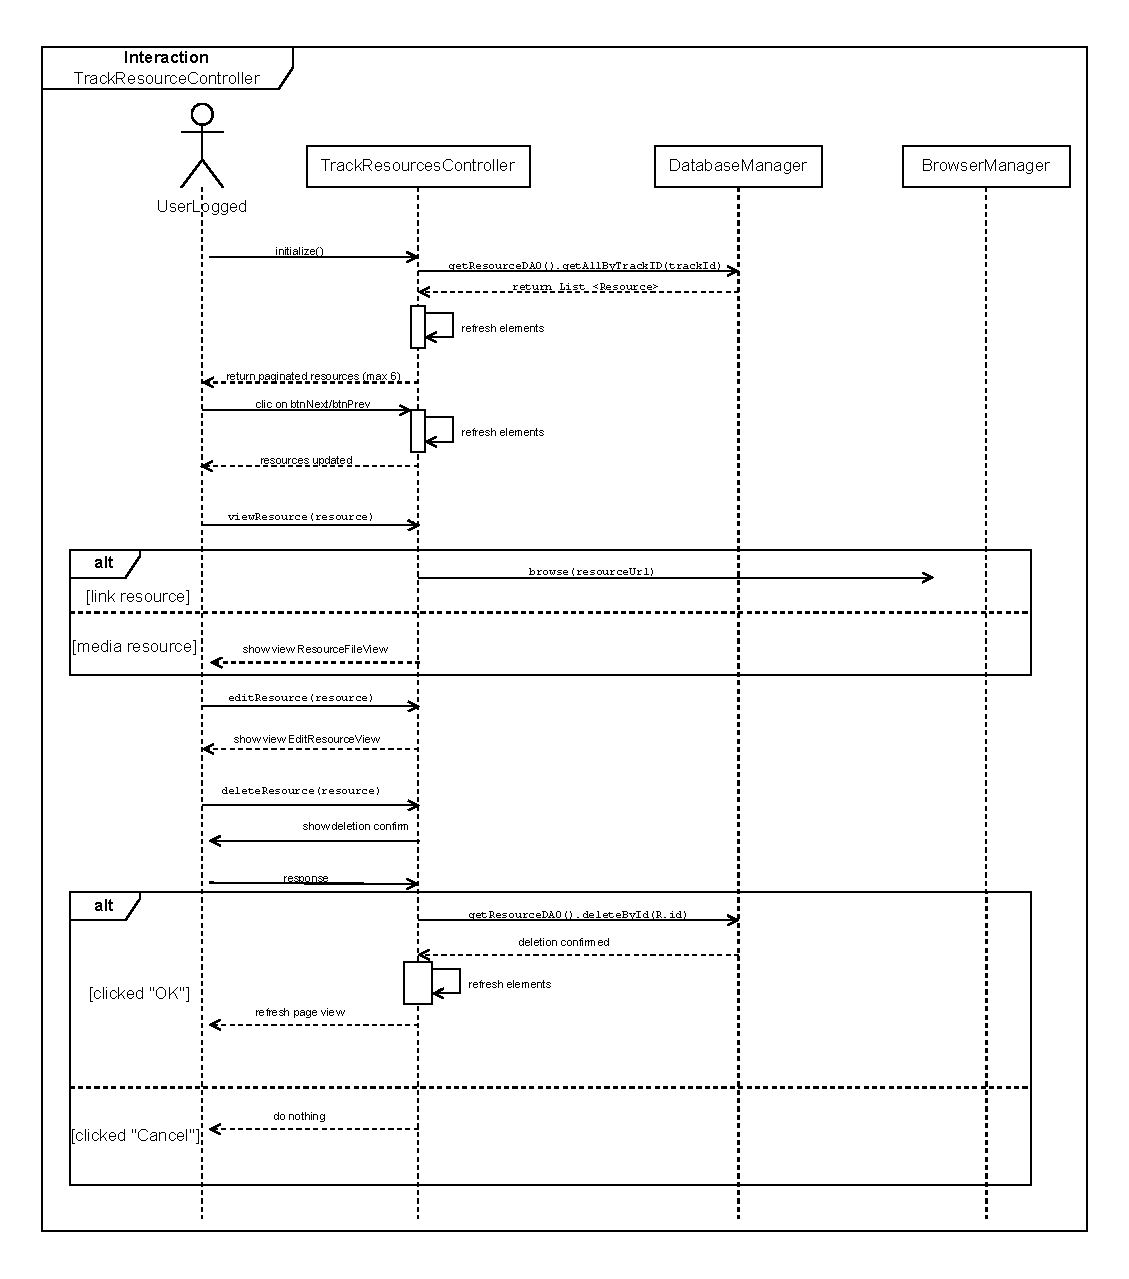
\includegraphics[width=0.8 \textwidth]{./figures/trackResourceController_sd}
    \caption{Sequence diagram relavito alla classe \texttt{TrackResourceController.java}}
    \label{fig:trackResourceController_sd}
\end{figure}

\begin{figure}[H]
    \centering
    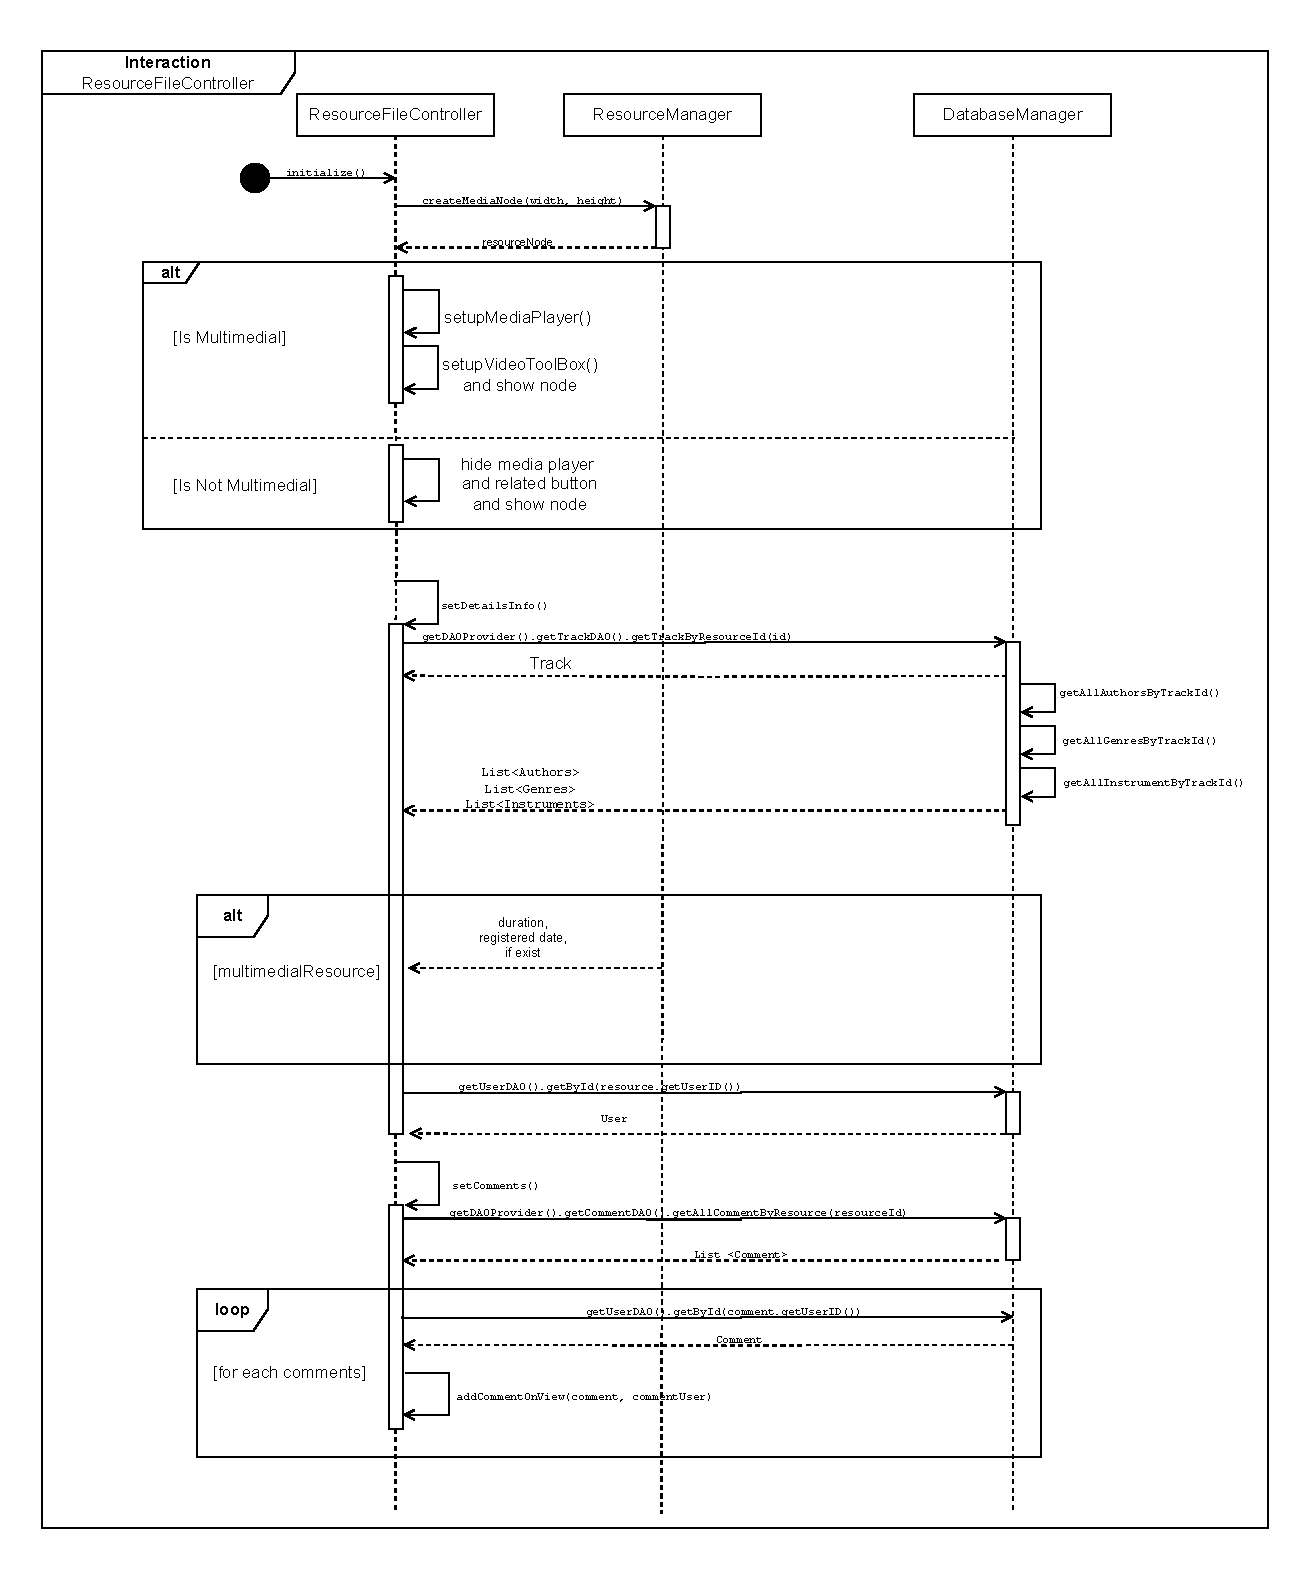
\includegraphics[width=0.8 \textwidth]{./figures/fileViewController_sd}
    \caption{Sequence diagram relavito alla classe \texttt{ResourceFileController.java}}
    \label{fig:resourcefilecontroller_sd}
\end{figure}



% =======================
\section{Progettazione e sviluppo}
% =======================

\subsection{Pattern utilizzati}
\subsubsection{Pattern architetturale}
Il sistema è stato progettato seguendo il pattern architetturale \textit{Model-View-Controller} (MVC), una struttura ampiamente adottata nello sviluppo di interfacce grafiche per separare le responsabilità delle diverse componenti software.

Il pattern MVC suddivide l'applicazione in tre componenti principali:

\begin{itemize}
    \item \textbf{Model}: rappresenta la logica e lo stato dell’applicazione. Contiene i dati, le classi di dominio e la logica di accesso ai dati (DAO), indipendente dalla logica di presentazione.

    \item \textbf{View}: è la parte visiva dell’applicazione, ovvero ciò che l’utente vede e con cui interagisce. In JavaFX, questa è rappresentata dai file \texttt{.fxml}, dai fogli di stile CSS e dai componenti grafici associati.

    \item \textbf{Controller}: gestisce l’interazione tra Model e View. Riceve gli input dell’utente dalla View, elabora le richieste e aggiorna il Model o la View di conseguenza. I controller in JavaFX implementano l’interfaccia \texttt{Initializable} per gestire l’inizializzazione della scena.
\end{itemize}

\bigskip

L'utilizzo del pattern MVC risulta particolarmente adatto in combinazione con JavaFX, poiché questa libreria supporta nativamente la separazione tra interfaccia grafica (FXML), logica di controllo (Controller) e dati (Model). In questo modo, il codice risulta più modulare, testabile e manutenibile.

\begin{figure}[H]
    \centering
    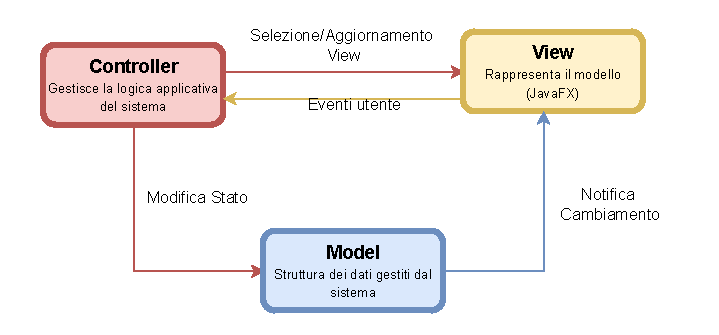
\includegraphics[textwidth]{./figures/mvc_template}
    \caption{Pattern MVC}
    \label{fig:mvc_template}
\end{figure}

\subsubsection{Design pattern utilizzati}
Durante lo sviluppo del progetto, si è deciso di adottare alcuni design pattern per migliorare la struttura e la gestione del codice. Tra questi:

\begin{itemize}
    \item \textbf{Singleton Pattern:} è un pattern creazionale che serve a garantire che una certa classe abbia una sola istanza. Ne sono un esempio tutte le classi del progetto denominate con \texttt{Manager} \texttt{(BrowserManager, ResourceManager ...ecc)}.

    \begin{figure}[H]
        \centering
        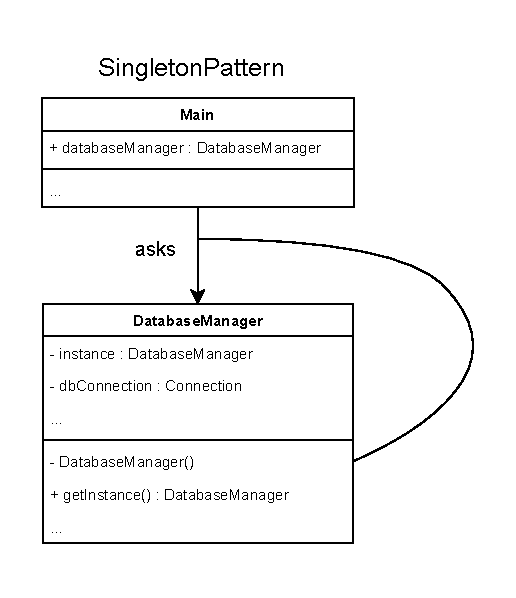
\includegraphics[\textwidth]{./figures/singletonPattern}
        \caption{Esempio Singleton Pattern riguardante la classe \texttt{DatabaseManager.java}}
        \label{fig:singleton_pattern}
    \end{figure}

    \item \textbf{Observer Pattern:} è un pattern comportamentale che si basa sul rapporto tra un oggetto osservatore e un oggetto osservato. L’osservatore si registra per essere notificato ogni volta che l’osservato cambia stato. In Java, questo pattern viene applicato implicitamente quando si lavora con strutture come \texttt{ObservableList}, molto usate per aggiornare automaticamente l’interfaccia utente in caso di modifiche. Ne sono un esempio tutti quei controlli utilizzati per filtrare, per esempio, le risorse o le tracce.

    \begin{figure}[H]
        \centering
        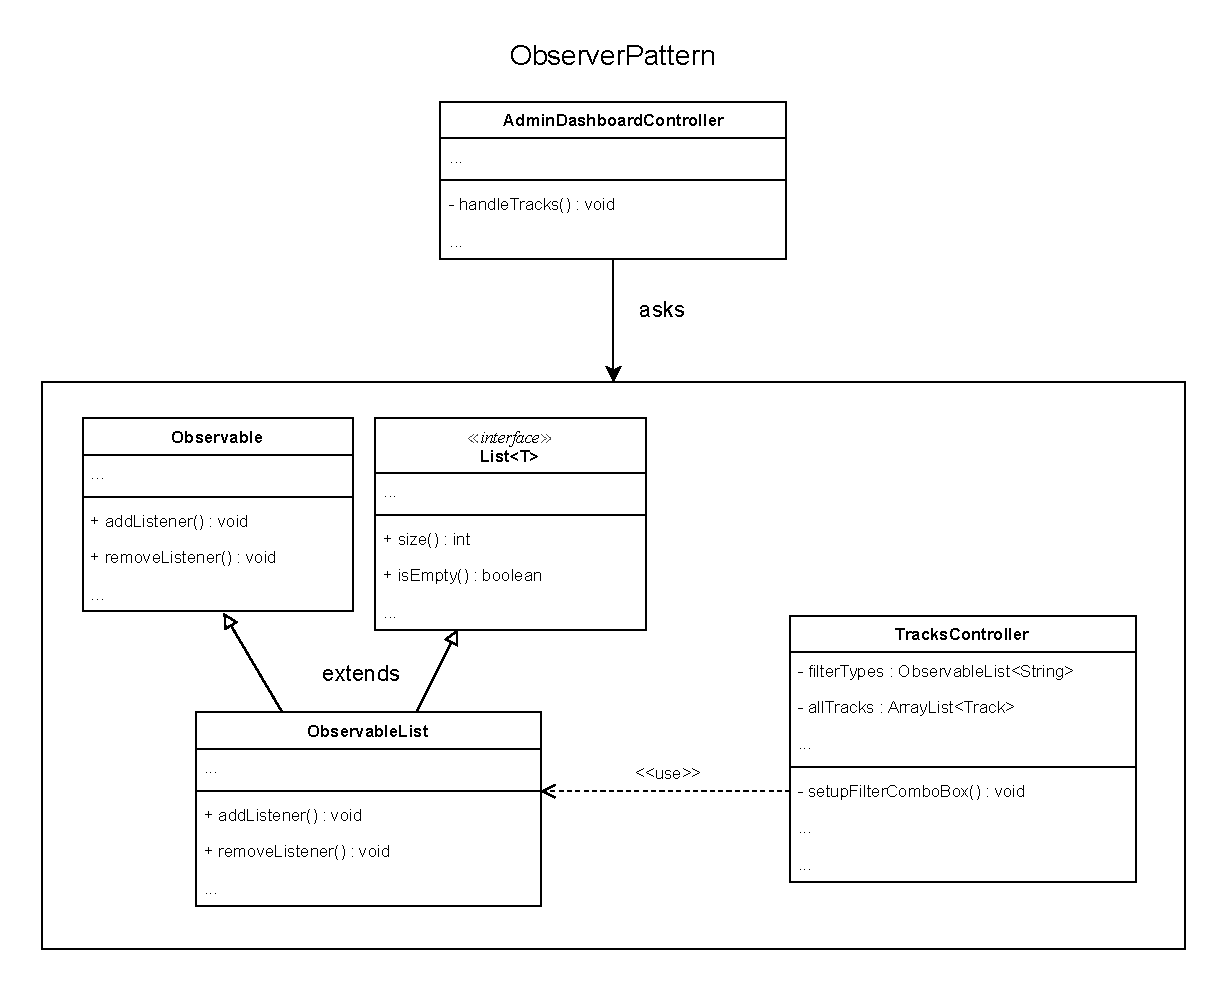
\includegraphics[width=0.8 \textwidth]{./figures/observer_pattern}
        \caption{Esempio Observer Pattern}
        \label{fig:observer_pattern}
    \end{figure}

    \item \textbf{Factory Pattern:} è un pattern creazionale che permette di delegare la creazione di un oggetto a un metodo preciso, senza specificare esattamente quale classe verrà istanziata. È stato utilizzato per la comunicazione tra due controller di due viste diverse, ad esempio, quando è necessario che un controller passi dei parametri ad un controller ad esso dipendente. Un esempio di codice utilizzato è il seguente (passaggio da lista di risorse a vista di una specifica risorsa):
    \begin{lstlisting}[style=java-style, caption={Esempio factory pattern}]
FXMLLoader loader = new FXMLLoader(...);
loader.setControllerFactory(_ -> new ResourceFileController(resource));
    \end{lstlisting}
    In questo caso, \texttt{FXMLLoader} gestisce internamente il factory pattern attraverso il metodo \texttt{setControllerFactory}.

    \begin{figure}[H]
        \centering
        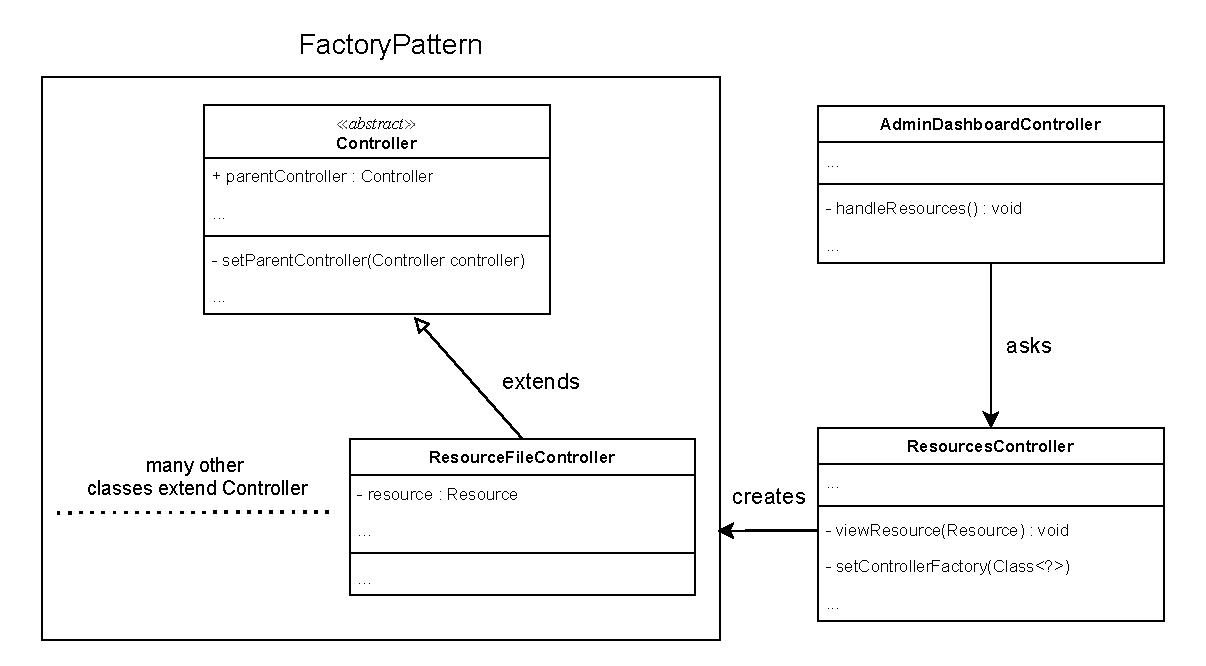
\includegraphics[width=0.8 \textwidth]{./figures/factory_pattern}
        \caption{Esempio Observer Pattern}
        \label{fig:factory_pattern}
    \end{figure}

    \item \textbf{DAO (Data Access Object) Pattern:} è un pattern strutturale che separa la logica di accesso ai dati dalla logica di business, e permette di fornire un'interfaccia di programmazione comune per le transazioni su database. Nel nostro caso, è stata definita un’interfaccia generica \texttt{DAO<T>} nel package \texttt{model}, che viene implementata da tutte le classi DAO. Ogni entità del modello è rappresentata come una semplice classe Java (POJO), che viene poi gestita dalla relativa implementazione DAO.

    \begin{figure}[H]
        \centering
        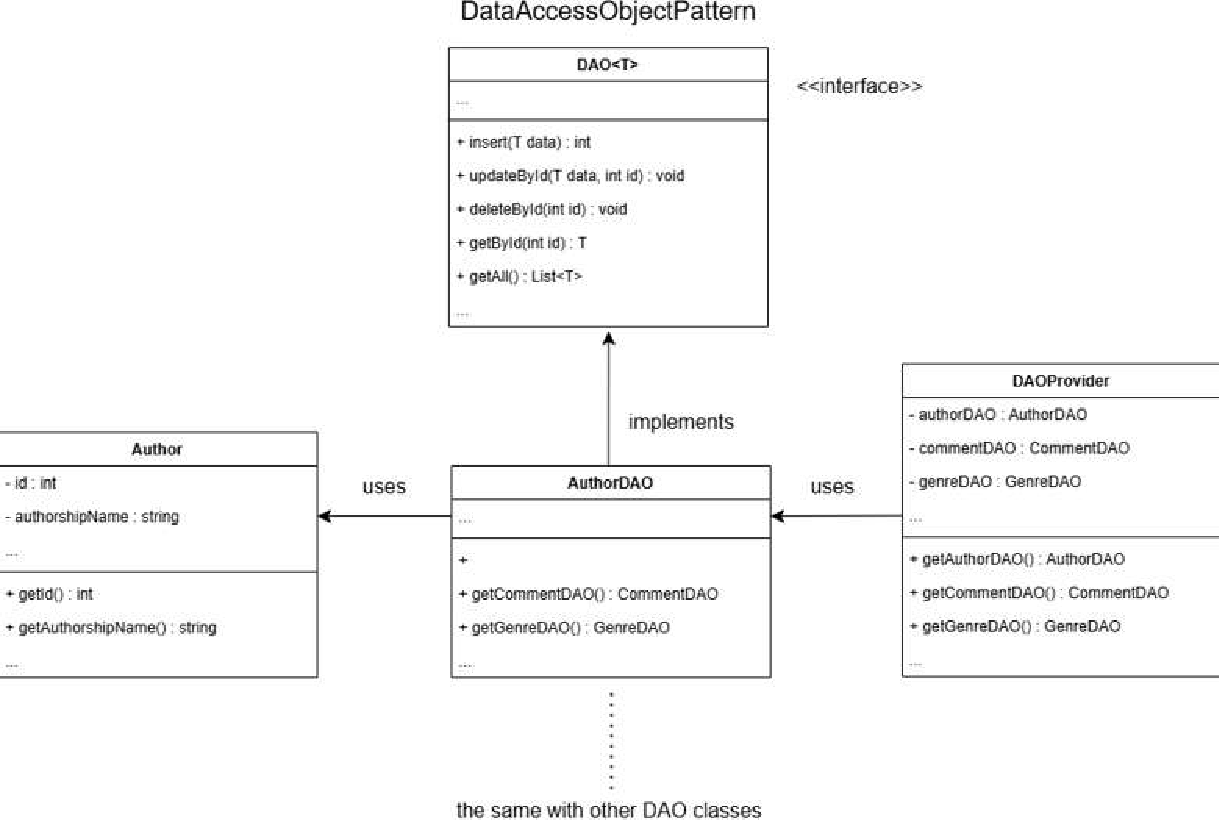
\includegraphics[width=0.8 \textwidth]{./figures/DAO_Pattern}
        \caption{Esempio DAO Pattern}
        \label{fig:DAO_Pattern}
    \end{figure}
\end{itemize}

\subsection{Gestione dell’accesso ai dati (DAO e DAOProvider)}
Il sistema adotta il pattern \textit{Data Access Object} (DAO) per gestire l’accesso ai dati in modo modulare e disaccoppiato dalla logica applicativa. Inoltre, abbiamo specificato operazioni ad hoc, in alcune classi DAO, in aggiunta a quelle dell'interfaccia comune, per facilitare alcune logiche di accesso che altrimenti sarebbero state pedanti.

L’accesso agli oggetti DAO all’interno dell’applicazione non avviene in modo diretto, ma è stato centralizzato attraverso una classe \texttt{"Wrapper"} denominata \texttt{DAOProvider}. Questo componente funge da punto di accesso unico (simile a un \textit{factory singleton}) per le istanze DAO, garantendo l'incapsulazione, una gestione coerente e facilitando eventuali modifiche future nel meccanismo di creazione o nella logica di accesso ai dati.

\subsection{Classi di supporto e utility}
Oltre alle classi principali legate al dominio e all’interfaccia utente, il sistema include alcune classi di supporto che forniscono funzionalità generiche e trasversali, riutilizzate in più parti del progetto. In questa sezione vengono descritte le principali classi di tipo \textit{utility} utilizzate.

\subsubsection{SessionManager}
La classe \texttt{SessionManager} si occupa della gestione della sessione utente all’interno dell’applicazione. Permette di salvare e recuperare rapidamente informazioni legate all’utente attualmente autenticato (es. ruolo, username, ID), rendendo disponibili questi dati ad altri componenti senza doverli passare esplicitamente.
La classe è implementata come \textbf{Singleton}, per garantire un’unica istanza condivisa.

\subsubsection{DBInit}
La classe \texttt{DBInit} è una classe utility responsabile della generazione dell'intera struttura del database SQLite.
Utilizza un approccio basato su stringhe statiche, compatibile con l'inizializzazione tramite la libreria SQLite, rendendo il processo più veloce e flessibile.
Include inoltre istruzioni per il controllo e l'inserimento dell'utente amministratore predefinito.
Il metodo \texttt{getDBInitStatement()} restituisce concatenati tutti i comandi SQL di creazione tabelle, utili per inizializzare il database in modo completo.

\subsubsection{SQLiteScripts}

La classe \texttt{SQLiteScripts}, anch'essa nel package \texttt{app.tracktune.utils}, fornisce metodi statici per gestire operazioni complesse o ricorrenti sul database.
Tra le principali funzionalità offerte troviamo:

\begin{itemize}
    \item \texttt{checkForSQLInjection(...)}: controlla se stringhe di input contengono pattern pericolosi riconducibili a SQL injection.
    \item \texttt{deleteTrack(...)}: esegue l'eliminazione completa e sicura di un brano, rimuovendo anche tutte le dipendenze correlate (commenti, risorse, interazioni, ecc.).
    \item \texttt{getMostRecentResources(...)}: restituisce le 5 risorse più recenti.
    \item \texttt{getMostPopularResources(...)}: ottiene le risorse più popolari, in base alla frequenza di appartenenza ai brani.
    \item \texttt{getMostCommentedResources(...)}: seleziona le risorse con il maggior numero di commenti.
\end{itemize}

% =======================
\section{Fase di Test}
% =======================
\subsection{Introduzione}
La fase di test ha lo scopo di verificare che il sistema sviluppato sia corretto, affidabile e conforme ai requisiti stabiliti.
Questa fase è essenziale per individuare eventuali errori o comportamenti inattesi prima della distribuzione finale del software.
I test sono stati suddivisi in più livelli:

\begin{itemize}
    \item \textbf{JUnit Test}: sono stati utilizzati per testare in modo automatico le unità di codice, in particolare metodi e classi del backend.

    \item \textbf{Test degli sviluppatori}: sono stati condotti test manuali durante lo sviluppo, volti a verificare il corretto funzionamento delle funzionalità implementate sia a livello logico che grafico. Questi test includono l’interazione con l’interfaccia grafica, la gestione degli errori e la validazione dei dati.

    \item \textbf{Test di utenti esterni}: una fase di test è stata dedicata all’interazione con utenti esterni al team di sviluppo, per raccogliere feedback sull’usabilità, sull’intuitività dell’interfaccia e sull’esperienza complessiva.
\end{itemize}


\subsection{JUnit Test}
Per la fase di test automatici è stato utilizzato il framework \textbf{JUnit}, che ha permesso di validare il corretto comportamento delle unità di codice in modo rapido e ripetibile. I test sono stati strutturati per coprire le principali funzionalità del sistema, con particolare attenzione alla correttezza logica dei metodi e alla gestione degli errori.

Le principali caratteristiche di JUnit impiegate sono state:

\begin{itemize}
    \item \textbf{Annotazioni}: sono state utilizzate annotazioni come \texttt{@Test} per definire i metodi di test, \texttt{@BeforeAll} per eseguire l'inizializzazione comune prima di tutti i test, e \texttt{@TestInstance} per permettere la condivisione dello stato tra i test all'interno della stessa classe.

    \item \textbf{Asserzioni}: sono state usate le principali asserzioni offerte da JUnit, tra cui \texttt{assertEquals}, \texttt{assertNotNull}, \texttt{assertTrue} e \texttt{assertThrows}, per verificare i valori attesi, la corretta creazione degli oggetti, la validità di condizioni booleane e il corretto lancio delle eccezioni.
\end{itemize}

\bigskip

I test sono collocati nella directory \texttt{test}, separata dal codice sorgente (\texttt{main}), così da mantenere indipendente la logica applicativa dal codice di test.
I test sono stati sviluppati in organizzati in package che rispecchiano la struttura del codice principale, ad esempio:
\begin{itemize}
    \item \texttt{app.tracktune.model.author} per quanto riguarda i test degli autori
    \item \texttt{app.tracktune.model.user} per quanto riguarda i test sugli utenti
    \item ecc
\end{itemize}

I test seguono un pattern comune:
\begin{itemize}
    \item \textbf{Setup}: Inizializzazione di un database SQLite in memoria per i test
    \item \textbf{Test CRUD}: Test per le operazioni Create, Read, Update, Delete
    \item \textbf{Test di relazioni}: Test per le relazioni tra entità (es. tracce-generi, tracce-autori)
\end{itemize}

Per i test viene utilizzato un database SQLite in memoria, in questo modo abbiamo un migliore isolamento tra software e test, impendeno qualunque effetto collaterale tra dati reali e di testing. Il database viene inizializzato tramite la classe \texttt{BBInit}

\begin{lstlisting}[style=java-style, caption={Esempio creazione database in memoria}]
// Esempio di inizializzazione del database per i test
String url = "jdbc:sqlite::memory:";
Connection connection = DriverManager.getConnection(url);
Statement stmt = connection.createStatement();
stmt.execute("PRAGMA foreign_keys = ON;");
String[] ddl = DBInit.getDBInitStatement().split(";");
for (String query : ddl) {
    if (!query.trim().isEmpty()) stmt.execute(query.trim() + ";");
}
\end{lstlisting}

Ogni classe DAO ha passato correttamente tutti i test, di seguito si riporta una classe di test come esempio:

\begin{lstlisting}[style=java-style, caption={Esempio test per la classe \texttt{UserTest.java}}]
import static org.junit.jupiter.api.Assertions.*;

@TestInstance(TestInstance.Lifecycle.PER_CLASS)
public class UserDAOTest {

    private UserDAO userDAO;

    @BeforeAll
    void setup() throws Exception {
        Connection connection = DriverManager.getConnection("jdbc:sqlite::memory:");
        try (Statement stmt = connection.createStatement()) {
            stmt.execute("PRAGMA foreign_keys = ON;");
            String[] ddl = DBInit.getDBInitStatement().split(";");
            for (String query : ddl) {
                if (!query.trim().isEmpty()) {
                    stmt.execute(query.trim() + ";");
                }
            }
        }
        DatabaseManager.setTestConnection(connection);
        DatabaseManager db = DatabaseManager.getInstance();
        userDAO = new UserDAO(db);
    }

    /**
     * Verifies the entry and retrieval of an AuthenticatedUser by ID.
     */
    @Test
    void insertAndGetById_AuthenticatedUser() {
        Timestamp now = new Timestamp(System.currentTimeMillis());
        AuthenticatedUser user = new AuthenticatedUser(null, "testUser", "password123", "Test", "User", UserStatusEnum.ACTIVE, now);
        Integer id = userDAO.insert(user);
        assertNotNull(id);

        User fetched = userDAO.getById(id);
        assertInstanceOf(AuthenticatedUser.class, fetched);
        AuthenticatedUser authUser = (AuthenticatedUser) fetched;
        assertEquals("testUser", authUser.getUsername());
        assertEquals("password123", authUser.getPassword());
        assertEquals("Test", authUser.getName());
        assertEquals("User", authUser.getSurname());
        assertEquals(UserStatusEnum.ACTIVE, authUser.getStatus());
        assertFalse(fetched instanceof Administrator);
    }

    /**
     * Verifies the entry and retrieval of an Administrator by ID.
     */
    @Test
    void insertAndGetById_Administrator() {
        Timestamp now = new Timestamp(System.currentTimeMillis());
        Administrator admin = new Administrator(null, "adminUser", "adminPass", "Admin", "User", UserStatusEnum.ACTIVE, now);
        Integer id = userDAO.insert(admin);
        assertNotNull(id);

        User fetched = userDAO.getById(id);
        assertInstanceOf(Administrator.class, fetched);
        Administrator fetchedAdmin = (Administrator) fetched;
        assertEquals("adminUser", fetchedAdmin.getUsername());
        assertEquals("adminPass", fetchedAdmin.getPassword());
        assertEquals("Admin", fetchedAdmin.getName());
        assertEquals("User", fetchedAdmin.getSurname());
        assertEquals(UserStatusEnum.ACTIVE, fetchedAdmin.getStatus());
    }

    /**
     * Verify the update of an existing AuthenticatedUser.
     */
    @Test
    void update_AuthenticatedUser() {
        Timestamp now = new Timestamp(System.currentTimeMillis());
        AuthenticatedUser user = new AuthenticatedUser(null, "updateUser", "initialPass", "Initial", "User", UserStatusEnum.ACTIVE, now);
        Integer id = userDAO.insert(user);

        AuthenticatedUser updated = new AuthenticatedUser(id, "updateUser", "updatedPass", "Updated", "User", UserStatusEnum.SUSPENDED, now);
        userDAO.updateById(updated, id);

        User result = userDAO.getById(id);
        assertInstanceOf(AuthenticatedUser.class, result);
        AuthenticatedUser authUser = (AuthenticatedUser) result;
        assertEquals("updateUser", authUser.getUsername());
        assertEquals("updatedPass", authUser.getPassword());
        assertEquals("Updated", authUser.getName());
        assertEquals(UserStatusEnum.SUSPENDED, authUser.getStatus());
    }

    /**
     * Verify the update of an existing Administrator.
     */
    @Test
    void update_Administrator() {
        Timestamp now = new Timestamp(System.currentTimeMillis());
        Administrator admin = new Administrator(null, "updateAdmin", "initialPass", "Initial", "Admin", UserStatusEnum.ACTIVE, now);
        Integer id = userDAO.insert(admin);

        Administrator updated = new Administrator(id, "updateAdmin", "updatedPass", "Updated", "Admin", UserStatusEnum.SUSPENDED, now);
        userDAO.updateById(updated, id);

        User result = userDAO.getById(id);
        assertInstanceOf(Administrator.class, result);
        Administrator fetchedAdmin = (Administrator) result;
        assertEquals("updateAdmin", fetchedAdmin.getUsername());
        assertEquals("updatedPass", fetchedAdmin.getPassword());
        assertEquals("Updated", fetchedAdmin.getName());
        assertEquals(UserStatusEnum.SUSPENDED, fetchedAdmin.getStatus());
    }

    /**
     * Verifies the deletion of a user by ID and that subsequent retrieval throws an exception.
     */
    @Test
    void deleteById_UserNotFound() {
        Timestamp now = new Timestamp(System.currentTimeMillis());
        AuthenticatedUser user = new AuthenticatedUser(null, "deleteUser", "password123", "Delete", "User", UserStatusEnum.ACTIVE, now);
        Integer id = userDAO.insert(user);

        userDAO.deleteById(id);

        assertThrows(app.tracktune.exceptions.SQLiteException.class, () -> userDAO.getById(id));
    }

    /**
     * Verify that the getAll method returns all users entered.
     */
    @Test
    void getAllUsers() {
        Timestamp now = new Timestamp(System.currentTimeMillis());
        AuthenticatedUser user1 = new AuthenticatedUser(null, "user1", "password1", "User", "One", UserStatusEnum.ACTIVE, now);
        Administrator admin1 = new Administrator(null, "admin1", "password2", "Admin", "One", UserStatusEnum.ACTIVE, now);
        userDAO.insert(user1);
        userDAO.insert(admin1);

        List<User> all = userDAO.getAll();
        assertTrue(all.size() >= 2);
        assertTrue(all.stream().anyMatch(u -> u.getUsername().equals("user1")));
        assertTrue(all.stream().anyMatch(u -> u.getUsername().equals("admin1")));
    }

    /**
     * Check recovery of an active user by username.
     */
    @Test
    void getActiveUserByUsername_ReturnsUser() {
        String uniqueUsername = "unique" + System.currentTimeMillis();
        Timestamp now = new Timestamp(System.currentTimeMillis());
        AuthenticatedUser user = new AuthenticatedUser(null, uniqueUsername, "password123", "Unique", "User", UserStatusEnum.ACTIVE, now);
        userDAO.insert(user);

        User fetched = userDAO.getActiveUserByUsername(uniqueUsername);
        assertNotNull(fetched);
        assertEquals(uniqueUsername, fetched.getUsername());
        assertEquals("Unique", fetched.getName());
        assertEquals("User", fetched.getSurname());
        assertInstanceOf(AuthenticatedUser.class, fetched);
        assertEquals(UserStatusEnum.ACTIVE, ((AuthenticatedUser) fetched).getStatus());
    }

    /**
     * Verifies that retrieving an inactive user by username returns null.
     */
    @Test
    void getActiveUserByUsername_InactiveUserReturnsNull() {
        String uniqueUsername = "inactive" + System.currentTimeMillis();
        Timestamp now = new Timestamp(System.currentTimeMillis());
        AuthenticatedUser user = new AuthenticatedUser(null, uniqueUsername, "password123", "Inactive", "User", UserStatusEnum.SUSPENDED, now);
        userDAO.insert(user);

        User fetched = userDAO.getActiveUserByUsername(uniqueUsername);
        assertNull(fetched);
    }
}
\end{lstlisting}

È possibile lanciare tutti i test con due metodologie:

\begin{itemize}
    \item Se Maven risulta correttamente installato all'interno del dispositivo, è possibile lanciare i test tramite:
    \begin{lstlisting}[style=bash-style, caption={Esecuzione test tramite Maven}]
mvn test
    \end{lstlisting}
    \item Tramite IDE (per quanto riguarda IntelliJ, recarsi nel menù laterale di destra $\rightarrow$ Maven $\rightarrow$ Lifecycle $\rightarrow$ test $\rightarrow$ run)
\end{itemize}

\subsection{Test degli sviluppatori}
In questa fase lo sviluppatore ha immesso nel sistema degli input (sia corretti che errati) per verificare se la reazione del software fosse quella attesa. Le funzionalità sono state testate man mano manualmente durante lo sviluppo, per assicurarsi che ogni componente rispondesse correttamente in base agli scenari previsti.

\subsection{Test di utenti esterni al sistema}
Per valutare la qualità, la chiarezza e l’usabilità del sistema da diversi punti di vista, sono stati coinvolti utenti esterni appartenenti a due categorie distinte:

\begin{itemize}
    \item \textbf{Utenti con competenze avanzate}: colleghi del corso di laurea in Informatica, con conoscenze tecniche in ambito software. Questi utenti hanno fornito feedback più approfonditi riguardo l’architettura, la fluidità dell’interfaccia e la coerenza del comportamento delle funzionalità. Sebbene non siano stati rilevati errori, il loro contributo è stato utile per confermare la solidità dell’applicazione anche in scenari di utilizzo meno comuni, oltre che per proporre miglioramenti specifici all’esperienza utente e alla gestione dei casi limite.

    \item \textbf{Utenti con competenze non avanzate}: amici e familiari privi di una formazione tecnica. In questo caso, il focus principale è stato posto sull’intuitività dell’interfaccia e sulla comprensibilità delle funzionalità offerte. I loro feedback si sono rivelati utili per verificare che l’utilizzo dell’applicazione fosse accessibile anche a un pubblico generalista, nonché per individuare eventuali errori o ambiguità.

\end{itemize}

I test sono stati svolti manualmente e in presenza, osservando il comportamento degli utenti durante l’interazione con il sistema e raccogliendo le loro impressioni immediate. Questo ha permesso di identificare aree migliorabili sia dal punto di vista tecnico che da quello dell’usabilità.
\end{document}
